%-----------------------------------------------------------------------
%                          hires2_correction.tex
% A&A LaTeX class (aa.cls)
%-----------------------------------------------------------------------
%\documentclass[referee]{aa}    % for a referee version
\documentclass{aa}
\usepackage{graphicx}
\usepackage{txfonts}
\usepackage{placeins}
\usepackage{natbib}
\usepackage[colorlinks,allcolors=blue,bookmarks=false]{hyperref}
\usepackage{xcolor}
\usepackage{amsmath}
\hyphenation{get-sources get-filaments get-images non-uniform back-ground}

\newcommand{\draftnote}[1]{\textcolor{magenta}{\textbf{[#1]}}}
\newcommand{\chg}[1]{\textcolor{magenta}{#1}}
\newcommand{\mH}{m_{\rm H}}
\newcommand{\muH}{\mu_{\rm H_2}}
\newcommand{{\um}}{\,$\mu$m}
\newcommand{\Teff}{T_{\rm E}}
\newcommand{\Sc}{\mathcal{D}_{\rm c}}
\newcommand{\Sim}{\mathcal{D}}
\newcommand{\Iim}{\mathcal{I}}
\newcommand{\Sig}{\Sigma}
\newcommand{\Ssh}{\Sigma_{\rm s}}
\newcommand{\Sbase}{\Sig_{\rm b}}

\begin{document}

\title{Correcting the temperature bias of dust surface density images\\of molecular clouds}

\author{Alexander Men'shchikov\inst{1}}
\institute{D\'epartement d'Astrophysique (DAp), IRFU, CEA Saclay,
Universit\'e Paris-Saclay, 91191 Gif-sur-Yvette, France}

\date{Received / Accepted}
\offprints{Alexander Men'shchikov}
\titlerunning{Correcting the temperature bias of surface density images}

\abstract{Surface densities of molecular clouds are obtained by fitting a single modified blackbody to the far-infrared intensities
of dust emission in each pixel. A line of sight crossing a dense structure is not isothermal, the fit is weighted toward the warmer
material, and the surface density is underestimated, by up to a factor of three in the densest material. The deficit cannot be
measured from the observed spectral energy distributions: its signature is 1 to 6\% of the intensities while the deficit itself is 9
to 38\%, so any scheme that infers one from the other amplifies photometric errors about eightfold. We therefore calibrate the
correction on radiative transfer models. A single relation between the dust temperature and the effective column of material that
shields it from the interstellar radiation field describes 102\,464 shells of 2086 models of embedded Bonnor--Ebert spheres, with a
mass-weighted scatter of 5.6\%. The shielding column is an average over the directions from which the radiation arrives, which makes
the result almost independent of the shape of the structure: a sphere, a cube and a plane-parallel layer of the same surface density
give correction factors within 10\% of one another. The correction factor follows as an explicit function of the surface density
that an image holds, with no fitted parameters, and it applies to a conventional surface density map as well as to every image of
the multi-resolution reconstruction produced by \emph{hires}. Tested on 1815 radiative transfer models that were not used in the
calibration, the correction raises the median core mass from 0.63 to 0.96 of the true value and the total surface density from
0.78 to 0.97, but a misjudgment of the footprint of a core by a quarter of its radius changes its mass by $-15$ to $+9$\%, more than
the correction leaves. On a simulated sky of cirrus, filaments and embedded cores, the flanks of filaments are over-corrected by up
to 30\%. The factor is calibrated for an interstellar radiation field of $G_0 = 10$, and models computed for $G_0 = 1$ to 500 show
that it over-corrects dense material by up to 33\% in weak fields and under-corrects it by up to 17\% in fields of a few tens.
Applied to a field of the Aquila cloud, the correction raises the integrated surface density by a factor of 1.66 and the number of
pixels above $10^{23}$\,cm$^{-2}$ ninefold.}

\keywords{ISM: clouds -- ISM: structure -- Stars: formation -- Infrared: ISM -- Submillimeter: ISM -- Techniques: image processing}

\maketitle
\nolinenumbers 

% =====================================================================

\section{Introduction}
\label{sec:intro}

Far-infrared and submillimeter surveys of molecular clouds with the \emph{Herschel} Space Observatory \citep{Pilbratt_etal2010}
have produced the images from which most of what is known about the structure of nearby star-forming regions has been derived
\citep[e.g.][]{Andre+2010, Konyves+2015, Andre+2014}. The physical quantity of interest, the surface density of dust and gas, is
not observed directly. It is obtained by fitting an optically thin modified blackbody to the intensities observed in each pixel
\citep{Hildebrand1983}, which yields one dust temperature and one surface density per line of sight.

Such images are the basis for the extraction of dense cores and filaments, and every quantity derived from them, in particular the
core mass function, inherits their accuracy. Their angular resolution is that of the longest waveband used, $36.3{\arcsec}$ at
500{\um}, unless a differential scheme transfers to them the higher resolution of the shorter wavebands
\citep{Palmeirim+2013}. The implementation used here, \emph{hires}, is described in \citet{Menshchikov2021method} and produces
surface density images at the resolution of any of the observed wavebands. The bias discussed below afflicts the conventional
image and the high-resolution one alike, since both rest on the same fit.

The single-temperature assumption is the weak point of the procedure. It is accurate for diffuse material, whose temperature varies
little along the line of sight, and it fails for a cold dense structure embedded in a warmer cloud. The fitted temperature is
weighted by the emission, hence by the warmer material, and the surface density derived from it is too low. The magnitude of the
effect follows from the logarithmic sensitivity of the Planck function,
\begin{equation}
   \frac{\partial \ln \Sig}{\partial \ln T} = -\,\frac{x_\lambda}{1-{\exp\left(-x_\lambda\right)}}\,, \quad
   x_\lambda \equiv \frac{h c}{\lambda k T}\,,
\label{eq:sensitivity}
\end{equation}
which at $T = 10$\,K equals $-8.99$ at 160{\um}, $-5.78$ at 250{\um}, $-4.18$ at 350{\um}, and $-3.05$ at 500{\um}. Overestimating
the dust temperature of a cold core by only 1\,K therefore lowers the surface density derived from the 500{\um} intensity by 30\%,
and the one derived from the 160{\um} intensity by a factor of 2.3. A modest error in the temperature is a large error in the
surface density.

The bias is not a multiplicative constant that could be absorbed into the assumed dust opacity. It grows with the surface density
of the surrounding cloud, because a denser environment produces a larger temperature contrast along the line of sight, and it grows
with the concentration of the structure, because a more centrally condensed core is more strongly shielded. Two structures of the
same true surface density, observed in different environments, are therefore recovered with different values, and their surface
densities are not comparable.

This paper presents a correction of that bias. It is a correction of an image and not of a particular way of making one: what it
needs is the surface density that a single modified blackbody fit returns at the resolution of the longest waveband, and that is
what any such image holds. The multi-resolution reconstruction is then an important special case rather than the subject, and a
useful one, because we show that the increments that a reconstruction adds at the finer resolutions are very nearly right, so that
the deficit is the same fraction of the surface density at every resolution and the factor can be evaluated on the image being
corrected.

Section~\ref{sec:where} shows why the deficit cannot be measured from the observed colors, and where in a reconstruction it
resides. Section~\ref{sec:law} derives, from a grid of radiative transfer models, the relation between the dust temperature and
the column that shields the material. Section~\ref{sec:corr} turns that relation into the correction and states what an image must
supply for it to be applied. Section~\ref{sec:valid} validates it on radiative transfer models that were not used in the
calibration and on a simulated sky, Sect.~\ref{sec:aquila} applies it to the Aquila cloud, and Sect.~\ref{sec:limits} states the
uncertainties, among which the dependence on the radiation field and the error of the background of a source.

Throughout this paper images are denoted by capital calligraphic characters, for instance $\Iim$ and $\Sim$, to distinguish them
from the scalar quantities that appear alongside them. Surface densities are given as the equivalent number of hydrogen molecules
per unit area, in cm$^{-2}$.

% =====================================================================

\section{Where the deficit resides}
\label{sec:where}

Two questions have to be settled before a correction can be constructed. The first is whether the observations themselves contain
the answer, so that the deficit of a line of sight could be read from the shape of its spectral energy distribution. They do not.
The mixing of temperatures along a line of sight broadens the spectral energy distribution only slightly: at the center of our
models, the residuals of a single modified blackbody fitted to the four wavebands are 1 to 6{\%} of the intensities, while
the fit loses 9 to 38{\%} of the surface density. A scheme that inferred the deficit from the residuals would therefore
amplify photometric errors by a factor of 7 to 9, which is far beyond the calibration accuracy of \emph{Herschel}, and the
correction has to be calibrated on models in which the answer is known (Appendix~\ref{app:colors}). The second question concerns
a multi-resolution reconstruction, which is not one image but a sequence of them: if the deficit were distributed differently over
the resolutions, each image would need its own correction. It is not, and that is what makes the high-resolution application as
simple as the conventional one.

\subsection{The multi-resolution reconstruction}
\label{sec:recon}

Let the observed wavebands be indexed by increasing wavelength $\lambda_i$ with beam half-maximum widths $\theta_i$, and let
$\mathcal{D}(\Iim, T, \lambda)$ denote the optically thin conversion of an intensity into a surface density at the wavelength
$\lambda$ and dust temperature $T$. Writing $G_{\theta_i \rightarrow \theta_{i+1}}$ for the Gaussian kernel that takes the beam
$\theta_i$ to the beam $\theta_{i+1}$, the reconstruction of \emph{hires} builds a base image at the coarsest resolution,
\begin{equation}
\Sim(\theta_N) = \mathcal{D}\!\left(\Iim_N^{\theta_N},\, T_N,\, \lambda_N\right),
\label{eq:base}
\end{equation}
where $T_N$ is the single dust temperature fitted at that resolution, and adds to it one increment per waveband,
\begin{equation}
\Delta_i = \max_{j}\Big[\,\mathcal{D}\!\left(\Iim_i^{\theta_i}, T_j, \lambda_i\right)
        - G_{\theta_i \rightarrow \theta_{i+1}} \ast \mathcal{D}\!\left(\Iim_i^{\theta_i}, T_j, \lambda_i\right)\Big],
\label{eq:increment}
\end{equation}
the maximum being taken over the resolutions at which a temperature is fitted. The image at any resolution is then the cumulative
sum
\begin{equation}
\Sim(\theta_i) = \Sim(\theta_N) + \sum_{i' \ge i} \Delta_{i'}\,.
\label{eq:cumulative}
\end{equation}
Equation~(\ref{eq:cumulative}) has a consequence that determines the design of the correction: an additive correction of the
base image corrects the image at every finer resolution by the same amount, without touching the increments.

\subsection{Decomposition of the deficit by scale}
\label{sec:deficit}

The true surface density decomposes in exactly the same way as Eq.~(\ref{eq:cumulative}), into a term convolved to the coarsest
beam and the differences between successive beams, so the two can be compared term by term. Table~\ref{tab:deficit} does this for
four radiative transfer models of a Bonnor--Ebert sphere embedded in a uniform cloud (Appendix~\ref{sec:grid}), summed over the
source mask at $36.3{\arcsec}$.

\begin{table}
\caption{Ratio of the reconstructed to the true surface density, term by term of Eq.~(\ref{eq:cumulative}), summed over the source
mask at $36.3{\arcsec}$, for four models with central-to-edge density ratios $\rho_{\rm c}/\rho_{\rm e}$. The rows give the base
image at $36.3{\arcsec}$, the sum of the three increments, and the total at $13.5{\arcsec}$. The increments are quoted as a
fraction of the total true surface density, since the true increments nearly cancel and their ratio is meaningless.}
\label{tab:deficit}
\centering
\begin{tabular}{lcccc}
\hline\hline
\noalign{\smallskip}
$\rho_{\rm c}/\rho_{\rm e}$    & 1.18   & 1.28   & 4.47   & 90.8   \\
\noalign{\smallskip}
\hline
\noalign{\smallskip}
base image at $36.3{\arcsec}$  & 0.967  & 0.946  & 0.797  & 0.819  \\
true increments                & 0.000  & 0.000  & 0.000  & 0.000  \\
recovered increments           & 0.021  & 0.025  & 0.026  & 0.006  \\
total at $13.5{\arcsec}$       & 0.988  & 0.970  & 0.824  & 0.825  \\
\noalign{\smallskip}
\hline
\end{tabular}
\end{table}

The true increments carry less than 2\% of the total surface density, because they are unsharp-masking terms whose integral over an
extended region very nearly cancels. The whole integrated deficit therefore resides in the base image. The reconstructed increments
do not cancel, because Eq.~(\ref{eq:increment}) clips them at zero at the shortest wavebands and takes a maximum over
temperatures, and they contribute a spurious positive excess three to six times the true one; that excess happens to act in the
right direction and repairs a few percent of the deficit.

Setting the base image to its true value and leaving the increments untouched would bring the integrated ratios of
Table~\ref{tab:deficit} from 0.988, 0.970, 0.824 and 0.825 to 1.021, 1.025, 1.026 and 1.006. The deficit is therefore carried by
the base image, and since the increments are nearly right, a finer image of the reconstruction holds the same deficit as the base
image at every scale that both contain. The correction can be formulated for the base image and added to the finer images, or
evaluated on a finer image directly; Sect.~\ref{sec:apply} describes both, and Sect.~\ref{sec:valid} compares them.

% =====================================================================

\section{What sets the temperature of the dust}
\label{sec:law}

\subsection{The radiation arrives from every direction}
\label{sec:why}

Dust in a molecular cloud is heated by the interstellar radiation field, the ultraviolet and optical light of the stars of the
Galaxy, which arrives from outside the cloud. A grain absorbs that radiation, warms up, and re-radiates in the far infrared, which
is what \emph{Herschel} observed. The temperature a grain settles at is therefore decided by how much radiation actually reaches
it, and that is diminished by the material lying between the grain and the outside.

The radiation arrives from all directions at once, and the material it must cross is different in each of them. Writing $I_0$ for
the unattenuated field, $\kappa$ for the opacity at the wavelengths that do the heating, and $\Sigma_{\rm a}(\hat n)$ for the
column of material the radiation traverses on its way in along the direction $\hat n$, the mean intensity reaching the grain is
\begin{equation}
J = \frac{1}{4\pi}\int I_0\,e^{-\kappa\,\Sigma_{\rm a}(\hat n)}\,{\rm d}\Omega .
\label{eq:meanint}
\end{equation}
We call $\Sigma_{\rm a}(\hat n)$ the attenuating column in the direction $\hat n$. It is a property of the incoming
radiation, not of anything leaving the cloud.

The upper panels of Fig.~\ref{fig:geometry} show what this means for the three shapes a cloud is usually described by. The arrows
are drawn thicker where the radiation has crossed less material, so that the eye sees which directions actually deliver energy.
Deep inside a layer the radiation arrives almost entirely along the normal, because a direction inclined by an angle $i$ has
crossed $1/\cos i$ times as much and grazing directions deliver nothing. At the center of a sphere every direction has crossed the
same column and none is favored. Inside a filament the two behaviors are combined: across the filament the path is short, along
its axis it is long, so a filament resembles a sphere in its cross section and a layer along its axis.

Rather than carry an integral over directions into every pixel, we replace the whole angular distribution by the single column
that would produce the same mean intensity. We call it the effective attenuating column $\Sigma_{\rm a}$ and define it by
\begin{equation}
e^{-\kappa\,\Sigma_{\rm a}} \;=\; \left\langle e^{-\kappa\,\Sigma_{\rm a}(\hat n)}\right\rangle_{4\pi} .
\label{eq:seff}
\end{equation}
It is larger than the column along the shortest path, because the oblique directions contribute less than that path alone would
suggest, and it is the quantity the dust temperature depends on.

\begin{figure*}
\centering
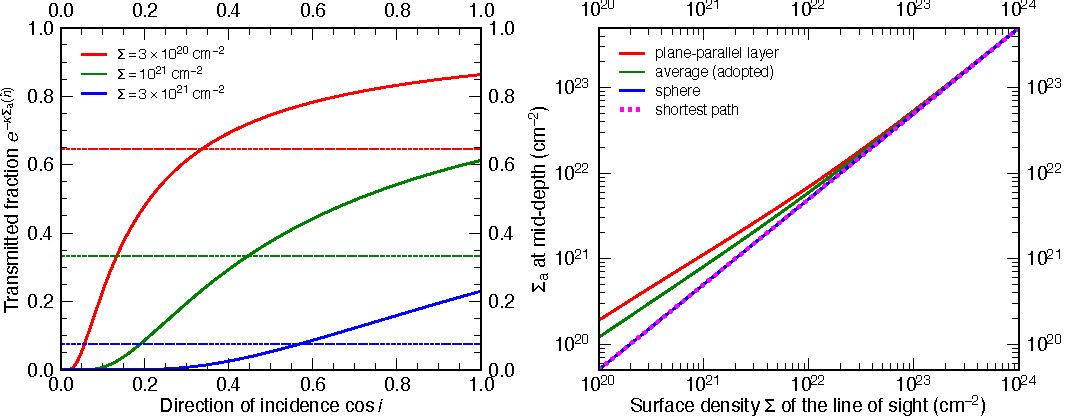
\includegraphics[width=0.85\textwidth]{fig_angular.pdf}
\caption{\emph{Left}: The fraction of the heating radiation that survives the journey inward, against the direction it comes from, 
for a parcel at mid-depth of a plane-parallel layer of three total surface densities. Plotted against the cosine of the angle, the
angular mean of each curve is the area beneath it, drawn dashed; the single column that would produce that same mean intensity is
the effective attenuating column of Eq.~(\ref{eq:seff}). \emph{Right}: that column against the total surface density of the line of
sight, for the two limiting shapes and for the average of them that is adopted, with the shortest path for comparison.}
\label{fig:angular}
\end{figure*}

Two assumptions are made here and should be stated plainly. The opacity at the heating wavelengths is taken as gray, with
$A_{\rm V} = N({\rm H_2})/0.94\times10^{21}$\,cm$^{-2}$ and $\tau = A_{\rm V}/1.086$; in reality it varies across the ultraviolet
and optical, so Eq.~(\ref{eq:seff}) is an average over wavelength as well as over direction. And the radiation field is taken to
be isotropic outside the cloud, which is what the models of Sect.~\ref{sec:models} assume.

\subsection{The models}
\label{sec:models}

The relation between the effective attenuating column and the dust temperature is not a free choice: it follows from radiative
transfer once the dust and the incident radiation field are fixed. We computed a grid of models with \emph{radmc-3d}
\citep{Dullemond+2012}, each a Bonnor--Ebert sphere \citep{Ebert1955, Bonnor1956} embedded in a uniform spherical cloud and heated
from outside by the interstellar radiation field, of strength $G_0 = 10$ in units of the local field, which includes the cosmic
microwave background. The dust opacity is that of \citet{Ossenkopf+Henning1994}, scaled to the power law $\kappa_\nu =
\kappa_0(\nu/\nu_0)^2$ with dust $\kappa_0 = 10.0$\,cm$^2$/g at $\nu_0 = 1000$\,GHz, a dust-to-gas mass ratio of $10^{-2}$ and
$\muH = 2.8$. The main grid holds 2089 models, which span the surface density of the embedding cloud, the size of the core and its
central-to-edge density ratio (Appendix~\ref{sec:grid}). Three of them, built to extend the grid to the highest surface densities,
are optically thick in the far infrared, a regime that the optically thin emission assumed by the correction does not describe, and
we leave them out of the calibration. The relation is fitted to the other 2086.

For every shell of every model the density structure is known, so the attenuating column can be computed along any direction by
integrating the density along that ray, and Eq.~(\ref{eq:seff}) evaluated by summing over directions. Shells are weighted by their
mass. Near the centers of the densest cores few photon packets of the Monte Carlo calculation arrive, and the temperatures of the
innermost cells scatter widely about the smooth profile; we reject a shell among the ten innermost ones when its temperature
departs by more than 10{\%} from the median of its five neighbors, together with every shell inside it. The rejected shells are
1.8{\%} of the total and hold a negligible fraction of the mass, so the fit does not depend on this choice.

\subsection{The relation}
\label{sec:relation}

The 102\,464 shells of the 2086 models fall on a single relation (Fig.~\ref{fig:shielding}), which we fit with
\begin{equation}
T(\Sigma_{\rm a}) = T_{\rm f} + (T_0 - T_{\rm f}) \left(1 + \frac{\Sigma_{\rm a}}{\Sigma_\star}\right)^{-\gamma},
\label{eq:law}
\end{equation}
$T_{\rm f} = 6.6304$\,K, $T_0 = 22.3710$\,K, $\Sigma_\star = 2.6469\times10^{21}$\,cm$^{-2}$ and $\gamma = 1.4392$, with a
mass-weighted scatter of 5.6{\%}. The two limits have simple meanings. $T_0$ is the temperature of dust that the radiation
field reaches unimpeded, and $T_{\rm f}$ the temperature it approaches when the radiation cannot reach it at all, the dust then
being warmed only by what little penetrates and by the microwave background. In bins of $\Sigma_{\rm a}$, the mass-weighted median
temperature of the models departs from the relation by less than 3.5{\%} up to $\Sigma_{\rm a} = 10^{23}$\,cm$^{-2}$; the
relation is 2 to 3.5{\%} too cold between $3\times10^{21}$ and $10^{23}$\,cm$^{-2}$ and exact below. Above
$10^{23}$\,cm$^{-2}$ the models hold too little mass to constrain it.

\begin{figure}
\centering
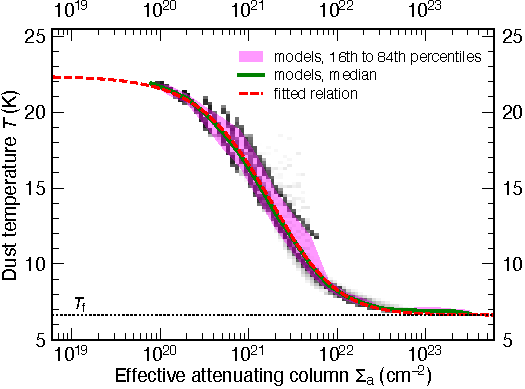
\includegraphics[width=0.9\columnwidth]{fig_shielding.pdf}
\caption{The dust temperature of the shells of 2086 radiative transfer models against their effective attenuating column. The
gray scale is the mass-weighted density of the shells, the solid line and band their weighted median and 16th to 84th percentiles
in bins of 0.2\,dex, and the dashed line the relation of Eq.~(\ref{eq:law}). The dotted line marks the temperature $T_{\rm f}$
approached by fully shielded dust.}
\label{fig:shielding}
\end{figure}

That one relation should describe models so different from one another is the result that makes the method possible, and it is
worth saying why it holds. Neither the size of the core nor its concentration appears in Eq.~(\ref{eq:law}), and neither needs to:
they act on the temperature only by changing how much material lies in the way of the radiation. The scatter about the relation,
5.6{\%}, measures how far structures of different shapes depart from it at the same attenuating column; it is physical and
would not decrease with more models.

% =====================================================================

\section{The correction}
\label{sec:corr}

\begin{figure*}
\centering
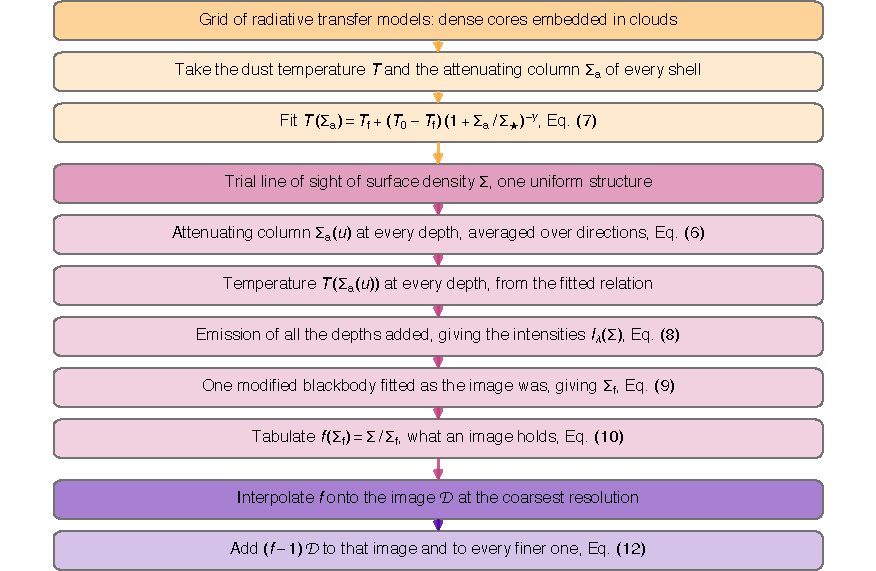
\includegraphics[width=0.75\textwidth]{fig_method.pdf}
\caption{The method step by step. The first group is the calibration, which is done once and yields the temperature relation of
Eq.~(\ref{eq:law}). The second is the calculation of Sect.~\ref{sec:factor}, repeated for every trial surface density, which
yields the table of the correction factor against the surface density that an observed image actually holds. The third is what is
then done to a reconstruction.}
\label{fig:method}
\end{figure*}

\subsection{The calculation}
\label{sec:factor}

Everything needed is now in place, and there is nothing left to adjust. For a line of sight of true surface density $\Sig$:
(\emph{i}) the effective attenuating column of the material at each depth is computed from Eq.~(\ref{eq:seff}), for a structure of
uniform density whose total surface density is $\Sig$; (\emph{ii}) its temperature follows from Eq.~(\ref{eq:law});
(\emph{iii}) the emergent intensity is the emission of all the layers added up,
\begin{equation}
   \Iim_\lambda(\Sig) = \kappa_\lambda\,\eta_{\rm dg}\,\muH\,\mH\,\Sig
   \int_0^1 B_\lambda \big(T(\Sigma_{\rm a}(u))\big)\,{\rm d}u ;
\label{eq:emission}
\end{equation}
(\emph{iv}) a single modified blackbody is fitted to it, in the same wavebands and with the same weights that the
reconstruction used, which gives a fitted temperature $\Teff$ and the surface density the reconstruction would report,
\begin{equation}
   \Sig_{\rm f}(\Sig) = \frac{\Iim_{\rm ref}(\Sig)} {\kappa_{\rm ref}\,\eta_{\rm dg}\,\muH\,\mH\,B_{\rm ref}(\Teff)} ;
\label{eq:fitted}
\end{equation}
(\emph{v}) the correction factor is the ratio, tabulated against $\Sig_{\rm f}$ because that, and not $\Sig$, is what an
observed image holds:
\begin{equation}
   f(\Sig_{\rm f}) = {\Sig}/{\Sig_{\rm f}} .
\label{eq:factor}
\end{equation}
Figure~\ref{fig:method} sets out the five steps together with what precedes and follows them.

\begin{figure}
\centering
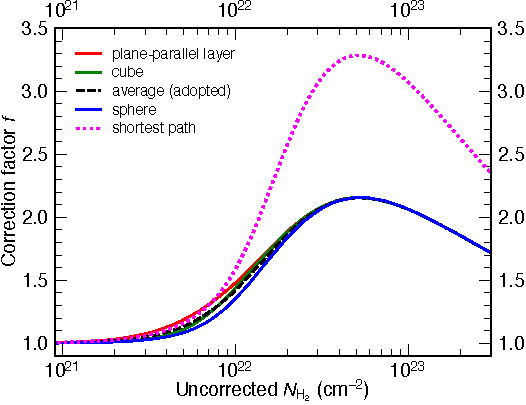
\includegraphics[width=0.85\columnwidth]{fig_relation.pdf}
\caption{The correction factor against the surface density of the uncorrected image, for a uniform plane-parallel layer, for a cube, 
for a uniform sphere, and for the average of the two that is adopted.}
\label{fig:relation}
\end{figure}

Figure~\ref{fig:relation} shows the result. The factor is unity below $10^{21}$\,cm$^{-2}$, where nothing is attenuated, rises
steeply through the range that most of a molecular cloud occupies, and flattens above $10^{23}$\,cm$^{-2}$, where the material is
against the temperature floor and no further shielding can cool it.

The lower panel of Fig.~\ref{fig:geometry} shows the quantity that drives the whole calculation, the run of $\Sigma_{\rm a}$ along
a line of sight. At $10^{21}$\,cm$^{-2}$ it is nearly flat, so the line of sight is nearly isothermal and there is almost nothing
to correct. As the surface density rises the profile steepens and approaches the dotted line, which is what the shortest path alone would
give: once the material is optically thick the oblique directions deliver nothing and only the normal matters.


\subsection{Why the shape hardly matters}
\label{sec:orient}

The calculation needs a shape, and an observed field does not supply one: cores are embedded in filaments, filaments are curved
and blended with their neighbors, and everything sits in a background that fluctuates on every scale. It is therefore important
that the answer should not depend much on which shape is assumed, and it does not.

Figure~\ref{fig:relation} gives the correction computed for a uniform sphere, a uniform cube and a uniform plane-parallel layer
of the same observed surface density. The three agree to within 10{\%} everywhere, and to 4{\%} or better outside a narrow band
near $10^{22}$\,cm$^{-2}$. The reason
is visible in Fig.~\ref{fig:geometry}: at low surface density nothing is attenuated and every shape gives unity, while at high surface density the
deepest material is optically thick in every direction and the distribution of path lengths ceases to matter. Sensitivity to shape
exists only in between, and there the correction itself is modest. Where the geometry would matter, the correction is small;
where the correction is large, the geometry does not matter. We average the sphere and the layer, and take their difference as the
uncertainty the geometry contributes.

Appendix~\ref{app:shape} explains why the sphere and the layer are the two limits, and why the angular average cannot be
replaced by the surface density along the shortest path.

One assumption remains, that each structure is of uniform density, and it matters far less than it appears. Along a
plane-parallel line of sight it does not matter at all. What shields a parcel of dust is the column of material lying between it
and the surface, and that column is what it is however the material within it is distributed: piling half of it into a dense
clump changes nothing about how much of it there is. The mass of a line of sight per unit column is constant as well, for any
density profile whatever, because the column is itself the integral of the density. Writing $\Sig(s)$ for the column in front of
a parcel at the depth $s$, the emission of Eq.~(\ref{eq:emission}) integrated along the line of sight is
\begin{equation}
   \int_0^L B_\lambda\big(T(\Sigma_{\rm a}(\Sig(s)))\big)\,\rho(s)\,{\rm d}s
   = \int_0^{\Sig} B_\lambda\big(T(\Sigma_{\rm a}(\Sig'))\big)\,{\rm d}\Sig' ,
\label{eq:invariance}
\end{equation}
and the density has disappeared. Two lines of sight of the same total surface density emit the same spectrum whether their material is
smooth or clumped, and whether a clump sits at the near face, in the middle or at the far face.
Appendix~\ref{app:arrange} confirms this numerically on density profiles differing by a factor of thirty, which reproduce the
smooth case to two parts in $10^{4}$.

Concentration and arrangement can therefore act only through the one thing that Eq.~(\ref{eq:invariance}) assumes, that the
radiation leaves along the line of sight rather than across it. They do, and by a modest amount. A sphere whose central-to-edge
density ratio is 10 requires a correction 3{\%} larger than a uniform sphere of the same central surface density, and one whose ratio
is $10^3$ requires between 6 and 15{\%} more, the difference growing with the surface density. A cirrus with a denser structure
embedded in it requires between 15{\%} less and 11{\%} more than the single uniform body that the method substitutes
for it, according to where within the cirrus the structure lies. Both are measured in Appendix~\ref{app:arrange} and enter the
budget of Sect.~\ref{sec:limits}.

\subsection{How it is applied}
\label{sec:apply}

The correction of an observed field requires one image of the reconstruction, the base image at some resolution $\theta_{\rm b}$:
\begin{equation}
\Sc(\theta_i) = \Sim(\theta_i) + \big[f\big(\Sim(\theta_{\rm b})\big) - 1\big]\,\Sim(\theta_{\rm b}) .
\label{eq:correction}
\end{equation}
The amount in brackets is computed once and added unchanged to the image at every resolution $\theta_i$, which
Eq.~(\ref{eq:cumulative}) permits because the increments do not depend on the base image. When the base is the image being
corrected, $\theta_{\rm b} = \theta_i$, Eq.~(\ref{eq:correction}) reduces to multiplying that image by $f$. We adopt the finest
image, $\theta_{\rm b} = 13.5{\arcsec}$, as the base. The factor was calibrated for the surface density that a single modified
blackbody fit returns at the resolution of the longest waveband, and the finest image is sharper than any such fit, so this
choice has to be justified by the tests of Sect.~\ref{sec:valid}: on the radiative transfer models it gives the most accurate
masses and profiles, and it also gives the sharpest corrected images. The base at $36.3{\arcsec}$ gives nearly the same masses and
remains a conservative alternative (Sect.~\ref{sec:base}). The correction is not idempotent, so it must be applied once; both of our
implementations stamp their output and refuse an input that has already been corrected.

\subsection{What the correction needs, and what it does not}
\label{sec:needs}

Nothing in Eqs.~(\ref{eq:seff}) to (\ref{eq:factor}) refers to the multi-resolution reconstruction. The factor is a function of
one number, the surface density that a single modified blackbody fitted to the observed intensities returns at the resolution of
the longest waveband, and that number can be obtained from the observed images alone. The base image of \emph{hires} is precisely
that fit and nothing else, which we verified directly on the grid: a single modified blackbody fitted here to the same wavebands
with the same weights reproduces the base image that \emph{hires} writes to better than 1{\%} at every node. The correction
therefore applies to a conventional surface density map made in the usual way from the \emph{Herschel} intensities convolved to a
common beam, whether or not \emph{hires} has been run, and Eq.~(\ref{eq:correction}) then reduces to multiplying that map by
$f$.

What the reconstruction supplies, and what no correction can replace, is the increments: the information on scales finer than the
longest waveband. Without them there is nothing at $13.5{\arcsec}$ to correct, and the corrected map is a map at
$36.3{\arcsec}$. The base image is therefore not an ingredient that has to be provided from outside; it is the anchor to which
the correction is attached, and it can be computed wherever the intensities are. The increments are the part that has to come
from somewhere else.

The order matters when the image is to be decomposed. The shielding of a parcel is set by the whole column along its line of sight,
so the factor has to be evaluated on the total surface density and not on any component of it. Correcting first and separating the
background afterwards recovers the crest of a filament above its background to 2{\%}; separating first and correcting the
background-subtracted structure, which evaluates the factor at a surface density the material does not have, recovers only 73{\%} of it. For
the same reason the correction must never be applied to an image that already carries it, nor to a true surface density: applying
the factor to the true image of the simulated sky would multiply the crest of a filament by a further 2.16.

One condition attaches to using the correction outside \emph{hires}. The table of $f$ is built for a particular set of wavebands
and a particular weighting of them, because the fitted surface density $\Sig_{\rm f}$ depends on both, and it must be rebuilt if
the map to be corrected was made from a different set or with different weights. It cannot, on the other hand, be replaced by
anything read from the photometry itself, for the reason given in Sect.~\ref{sec:amplification}: the signature of the temperature
mixing lies below the calibration uncertainties, so the correction has to come from the models whatever image it is applied to.

Two further properties follow immediately from the construction. The correction is insensitive to noise, because it evaluates a
smooth function of an image rather than fitting anything: adding Gaussian noise of 1.5, 0.50, 0.30 and
0.15\,MJy\,sr$^{-1}$ at 160, 250, 350 and 500{\um} changes the integrated corrected surface density of the models by less than
0.5\%. And it depends on the
photometric calibration of the reference waveband only, in exact proportion, because the base image is proportional to that one
intensity; the amplification by 8 to 10 found in Sect.~\ref{sec:amplification} does not apply, since the colors are not used.

% =====================================================================


\section{Validation}
\label{sec:valid}

A correction can be tested only where the true surface density is known. We test it in two settings that complement each other.
The radiative transfer models are exact, but each holds a single core in a smooth cloud. The simulated sky of
Sect.~\ref{sec:sim} holds cores, filaments and a diffuse cirrus along the same lines of sight, but its temperatures follow the
relation of Eq.~(\ref{eq:law}) rather than a radiative transfer calculation, so it cannot reveal an error in that relation.

\subsection{On the radiative transfer models}
\label{sec:valgrid}

The relation of Eq.~(\ref{eq:law}) was fitted to the models of the main grid. To test the correction on models that played no
part in the fit, we computed a second grid of 1815 models whose parameters lie between those of the main grid, in the same
radiation field of $G_0 = 10$ (Appendix~\ref{sec:grid}). For each model, the emission was convolved to the beams of the four
wavebands, reconstructed by \emph{hires} as an observation would be, and corrected with the base image at $13.5{\arcsec}$ and,
for comparison, at $36.3{\arcsec}$. The corrected images are compared with the true surface density of the model at the same
resolution in three ways, and Table~\ref{tab:valgrid} gives the results.

The first measure is the total surface density within the footprint of the model, the area where the model stands above its
surroundings in the true image at $13.5{\arcsec}$, divided by the same total in the true image. It shows whether the correction
restores the right amount of material. The second is the mass of the core. It is the same total with the background subtracted,
where the background is the median surface density in a ring $15{\arcsec}$ wide just outside the footprint, and it is again
divided by the same measurement on the true image. The third is the radial profile of the relative residual, the corrected minus
the true surface density divided by the true surface density, as a function of the distance from the center of the core. Each
measure is computed for every model, and Table~\ref{tab:valgrid} gives the median over the models with the 16th and 84th
percentiles, which bracket the central 68{\%}.

\begin{table}
\caption{Validation on 1815 radiative transfer models that were not used to fit the relation of Eq.~(\ref{eq:law}). Total:
the surface density summed over the footprint of the model, divided by the true value. Core mass: the same sum less the
background, divided by the same measurement on the true image. Center and $21{\arcsec}$: the relative residual of the surface
density at 3 and $21{\arcsec}$ from the center of the core. The first two columns give the median over the models, with the 16th
and 84th percentiles in parentheses; the last two give medians.}
\label{tab:valgrid}
\centering
\begin{tabular}{lcccc}
\hline\hline
\noalign{\smallskip}
\!\!\! Image & \!\!\!\! Total & \!\!\!\! Core mass & \!\!\!\!\! Center & $21{\arcsec}$\!\!\\
\noalign{\smallskip}
\hline
\noalign{\smallskip}
\!\!\! uncorr.              & \!\!\!\!\! 0.78 (0.56--0.93) & \!\!\!\!\! 0.63 (0.46--0.86) & \!\!\!\!\!\!\! $-0.44$ & \!\!\!\!\!\!\! $-0.21$\!\!\\
\!\!\! base $36.3{\arcsec}$ & \!\!\!\!\! 0.96 (0.89--1.00) & \!\!\!\!\! 0.94 (0.70--1.09) & \!\!\!\!\!\!\! $-0.15$ & \!\!\!\!\!\!\! $-0.01$\!\!\\
\!\!\! base $13.5{\arcsec}$ & \!\!\!\!\! 0.97 (0.91--1.00) & \!\!\!\!\! 0.96 (0.74--1.14) & \!\!\!\!\!\!\! $-0.12$ & \!\!\!\!        $0.00$\!\!\\
\noalign{\smallskip}
\hline
\end{tabular}
\end{table}

\begin{figure*}
\centering
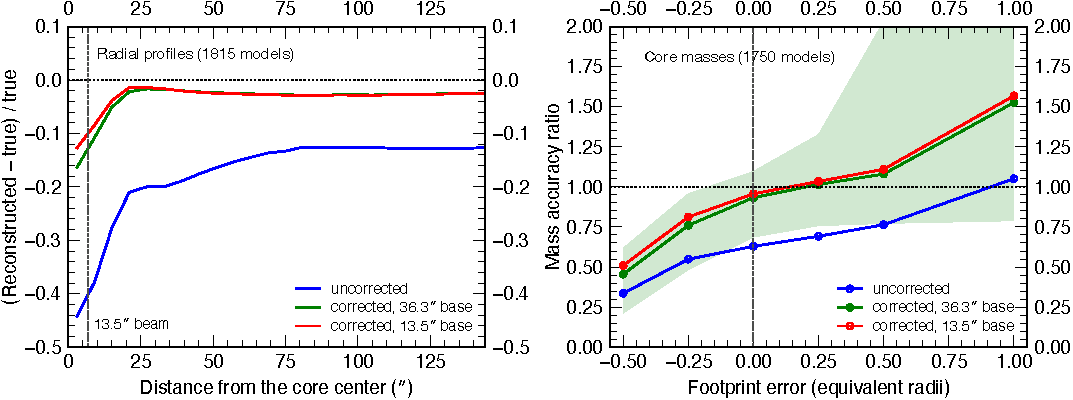
\includegraphics[width=0.9\textwidth]{fig_grid_validation.pdf}
\caption{The correction tested on 1815 radiative transfer models that were not used to fit the relation of
Eq.~(\ref{eq:law}). \emph{Left}: the relative residual of the surface density, the reconstructed minus the true value divided by
the true value, against the distance from the center of the core, as the median over the models. The dashed line marks half the
beam of $13.5{\arcsec}$. \emph{Right}: the mass of the core, divided by the true mass, when the footprint within which it is
measured is too small (negative abscissa) or too large (positive abscissa) by the given fraction of its equivalent radius. The
background is always taken in a ring just outside the footprint used. The lines are medians over the models, and the band marks
the 16th to 84th percentiles for the correction with the base at $36.3{\arcsec}$.}
\label{fig:valgrid}
\end{figure*}

Uncorrected, the reconstruction holds 78{\%} of the true surface density and 63{\%} of the mass of the core, and the
deficit is largest at the center, where it reaches 44{\%}. The correction restores the total to 97{\%} and the mass of
the core to 96{\%} in the median. Beyond $20{\arcsec}$ from the center, the residual is within 2.5{\%} at all
distances (Fig.~\ref{fig:valgrid}, left). What remains is a deficit at the center of the core, 12{\%} at $3{\arcsec}$, which
is the part of the error that no correction depending on the surface density alone can remove: the center of a core is colder
than the center of a uniform structure with the same surface density, and nothing in the surface density reveals it. The base at
$36.3{\arcsec}$ gives almost the same totals but a larger deficit at the center, because the factor it applies varies more
slowly than the core it corrects (Sect.~\ref{sec:base}).

The spread over the models is larger than any of these medians. For one core in six the corrected mass is more than a quarter
below the true one, and for one in six it is more than 14{\%} above it. A correction that depends on the surface density
alone cannot remove this spread, because models with the same surface density can differ in how their temperature varies along
the line of sight.

\paragraph{The footprint matters more than the correction.}
In a real image, the footprint of a core is not known and has to be estimated, together with the background beneath it. The
right panel of Fig.~\ref{fig:valgrid} shows what an error in the footprint does to the measured mass. A footprint too small by a
quarter of its radius lowers the median mass of the corrected image from 0.96 to 0.82 of the truth, and one too small by half its
radius lowers it to 0.51, because part of the core is then counted as background. A footprint too large by a quarter or a half of
its radius raises the median mass to 1.05 or 1.14, and the spread over the models widens sharply. These errors are lower limits,
because the models sit in a cloud of uniform density, whose surface density declines smoothly with radius; a real core is
surrounded by filaments and other cores, which enter a background ring in ways no model reproduces.

The correction thus removes a systematic deficit of about 40{\%} in the masses of cores, and what it leaves, a few percent
in the median, is smaller than the error that a plausible misjudgment of the footprint and background introduces. We return to
this in Sect.~\ref{sec:limits}.

\subsection{On a simulated sky}
\label{sec:sim}

The models of Sect.~\ref{sec:valgrid} are single spheres, and an observed field is not. We therefore built a simulated sky
containing a diffuse cirrus, seven filaments and 96 embedded cores, in which the true surface density is known by construction. The
cirrus is plane-parallel and the filaments are cylinders with the cross-section observed in real clouds, a width of $40{\arcsec}$
and wings falling as $r^{-0.75}$; their temperatures follow Eq.~(\ref{eq:law}) with the geometry of each component. The cores are
radiative transfer models of the grid, with known masses. The intensities were computed at 70 to 500{\um}, convolved to the
corresponding beams, sampled on $3{\arcsec}$ pixels and passed through \emph{hires} exactly as an observation would be. In a second
version of the sky, the filaments are inclined at random to the plane of the sky, which leaves their surface density unchanged but
changes how strongly they are shielded.

The sky tests what the models cannot, the superposition of several structures along a line of sight, but it has a limitation of
its own: its filaments and cirrus obey Eq.~(\ref{eq:law}) by construction, and a pixel that holds several of them is warmer than a
single body of the same total surface density. A correction that assumes a single body over-corrects such pixels
(Appendix~\ref{app:arrange}), so the sky measures that bias together with the accuracy of the correction.

\begin{table}
\caption{Fraction of the true value recovered on the simulated sky at $13.5{\arcsec}$, before the correction and after it with the
base image at $13.5{\arcsec}$ (the adopted one) and at $36.3{\arcsec}$, for filaments in the plane of the sky and inclined at
random. Total: the surface density summed over the field. Core center: the central pixel of each core. Core mass: the surface
density within one Bonnor--Ebert radius less the background measured between 2 and 2.5 radii, divided by the same measurement on
the true image. The core entries are medians over the cores.}
\label{tab:sim}
\centering
\begin{tabular}{llccc}
\hline\hline
\noalign{\smallskip}
Sky & Quantity & Uncorr. & Base $13.5{\arcsec}$ & Base $36.3{\arcsec}$ \\
\noalign{\smallskip}
\hline
\noalign{\smallskip}
plane    & total       & 0.776 & 1.133 & 1.106 \\
         & core center & 0.542 & 1.064 & 1.010 \\
         & core mass   & 0.566 & 1.096 & 1.006 \\
inclined & total       & 0.788 & 1.160 & 1.133 \\
         & core center & 0.553 & 1.064 & 1.010 \\
         & core mass   & 0.561 & 1.088 & 1.008 \\
\noalign{\smallskip}
\hline
\end{tabular}
\end{table}

\begin{figure*}
\centering
\includegraphics[width=\textwidth]{fig_simsky.pdf}
\caption{A part of the simulated sky at $13.5{\arcsec}$: the reconstruction of \emph{hires}, the same image after the correction
of Eq.~(\ref{eq:correction}), and the true surface density. The three panels share one logarithmic scale.}
\label{fig:simsky}
\end{figure*}

\begin{figure}
\centering
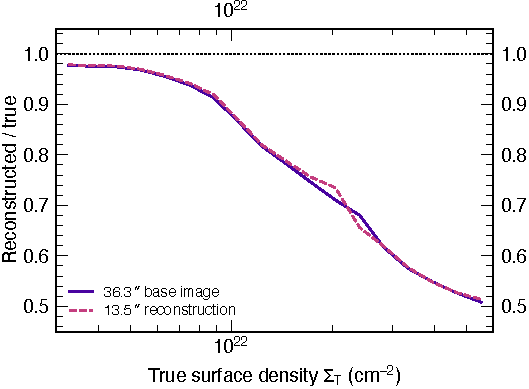
\includegraphics[width=0.9\columnwidth]{fig_deficit.pdf}
\caption{The reconstruction of the simulated sky divided by its true surface density, in bins of the true surface density, at the
coarsest resolution and at the finest. The two curves lie almost on top of one another: the increments that the reconstruction
adds between those resolutions are very nearly right, and the deficit is the same fraction of the surface density at both
resolutions.}
\label{fig:deficit}
\end{figure}

Figure~\ref{fig:simsky} shows the sky before and after correction beside the truth, and Table~\ref{tab:sim} gives the numbers.
Before the correction, the reconstruction holds 78{\%} of the true surface density, 54{\%} at the centers of the cores
and 57{\%} of their masses. After it, the masses of the cores come out 9 to 10{\%} too high with the adopted base and
within 1{\%} with the base at $36.3{\arcsec}$, and the total 13 to 16{\%} too high with either. The excess of the total
is the superposition bias described above: most of the area of the field is diffuse, and its cirrus and filaments shield each
other less than the single body that the correction assumes. The cores of the sky sit on that over-corrected background, and on
the models, where each core sits in its own smooth cloud, the same correction gives masses 4{\%} too low
(Sect.~\ref{sec:valgrid}). The two tests thus bracket the truth, and neither offset is large compared with the error of the
background of Sect.~\ref{sec:valgrid}. Figure~\ref{fig:deficit} shows, on the simulated sky, the property derived on the models in
Sect.~\ref{sec:deficit}: the reconstruction falls below the truth by the same fraction at both resolutions at every surface
density, so the factor can be evaluated at either.

\subsection{Where the correction fails}
\label{sec:fails}

\begin{figure*}
\centering
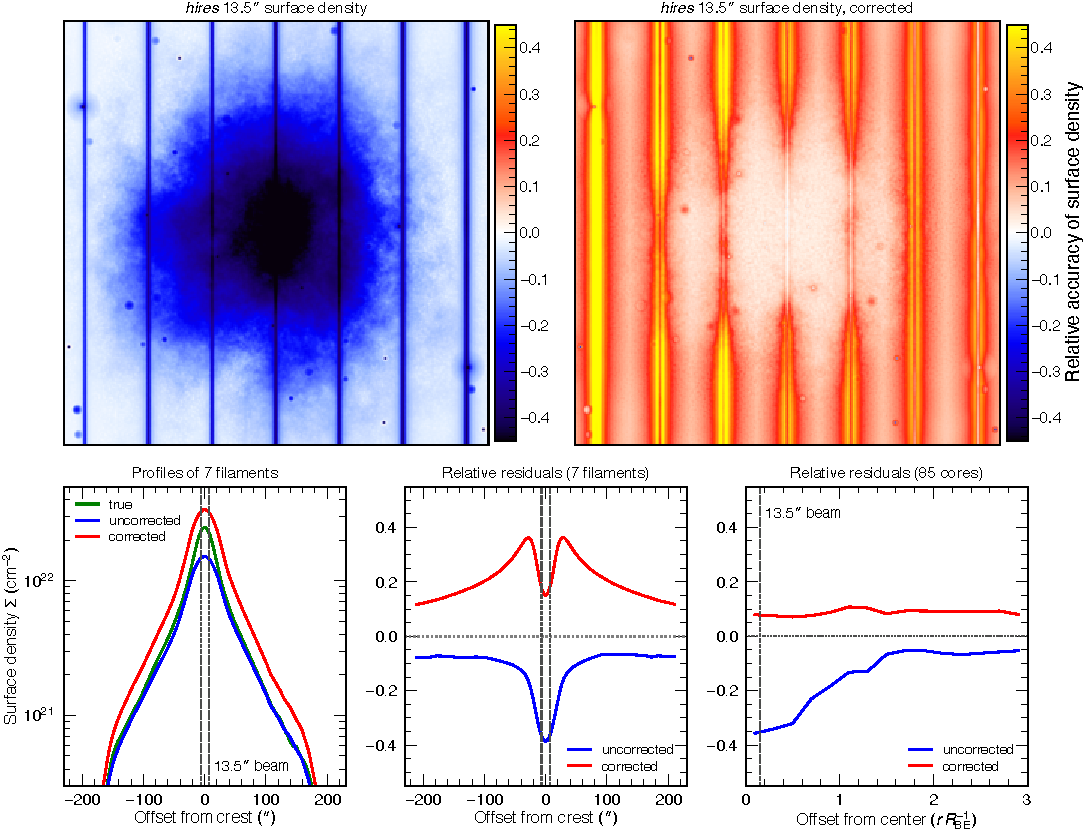
\includegraphics[width=\textwidth]{fig_simsky4_residual.pdf}
\caption{\emph{Upper panels}: the relative residual of the reconstruction at $13.5{\arcsec}$ against the true surface density of
the simulated sky, before and after the correction, on the same scale. \emph{Lower panels}: the profiles themselves, stacked over
the seven filaments and with their backgrounds removed; the same profiles as relative residuals; and the residual stacked over the
injected cores against the radius in units of the Bonnor--Ebert radius. The dashed lines mark the $13.5{\arcsec}$ beam.}
\label{fig:residual}
\end{figure*}

The numbers of Table~\ref{tab:sim} are averages, and Fig.~\ref{fig:residual} shows what they average over. Before the correction
the reconstruction is too low everywhere: by about 10{\%} over the diffuse field and by 40{\%} at the centers of the
cores and at the crests of the filaments. After it, the crests of the filaments are within 6 to 12{\%} of the truth, but the
flanks of the filaments are over-corrected by up to 30{\%} some $20{\arcsec}$ from the crest, and a weaker ring of
over-correction surrounds the cores.

The reason is that the factor is a function of the observed surface density and of nothing else. The shielding of a filament
falls with the distance from its axis much faster than the shielding of a uniform body falls with its surface density. On the
axis, a filament is shielded by about half of its surface density, close to what a uniform body of that surface density would
give, so its crest comes out right. Away from the axis, the surface density is still high, but the material there lies near the
surface of the filament and is barely shielded; a uniform body of that surface density would be much colder, and the correction
applied there is too large. The rings around the cores are the same effect for a sphere. The inclination of a filament acts in the
same direction: a filament seen obliquely presents a larger surface density than its radius shields, and on the inclined sky the
crests are over-corrected by 6 to 45{\%}, the more the further a filament is inclined from the plane of the sky.

No correction that depends on the surface density alone can remove this, because it cannot distinguish a given surface density
on the flank of a filament from the same surface density in the body of a uniform structure. We tested corrections that use the
fitted temperature as a second observable, calibrated on the radiative transfer models; they fail for a reason that is instructive
and is described in Appendix~\ref{app:tcorr}. What the flanks do to the widths, slopes and linear density of filaments is
quantified in Appendix~\ref{app:filaments}. In short, the correction restores the logarithmic slope of the wings of a filament,
from 0.57 to 0.75 against a true 0.82, but a filament remains 44{\%} too wide after the correction, as it was 86{\%} too
wide before it, and its linear density comes out 35 to 55{\%} too high.

\subsection{The choice of the base image}
\label{sec:base}

Nothing in Sect.~\ref{sec:corr} ties the correction to one resolution, and Fig.~\ref{fig:base} in Appendix~\ref{app:filaments}
shows what the choice of the base image changes. A finer base gives a correction that follows the structures more closely: the
width of a filament comes down from 78 to $72{\arcsec}$ and the index of its wings rises from 0.73 to 0.75, against a true
$50{\arcsec}$ and 0.82. On the simulated sky it raises the masses of the cores by about 9{\%}, and on the radiative transfer models
by 3{\%}, which there brings them closer to the truth (Table~\ref{tab:valgrid}). The two bases differ by less than the error of the
background, and we adopt the finest one, which gives the sharper images; the base at $36.3{\arcsec}$ remains a conservative
alternative, useful when a corrected map at the resolution of the longest waveband is wanted, since it then reduces to multiplying
a conventional surface density map by $f$.

% =====================================================================

\section{Application to the Aquila cloud}
\label{sec:aquila}

We applied the correction to a $31\arcmin \times 31\arcmin$ field of the Aquila cloud observed with \emph{Herschel} at 70,
160, 250, 350 and 500{\um} \citep{Andre+2010, Konyves+2015}, adopting a distance of 260\,pc. The factor is evaluated on the
reconstruction at $13.5{\arcsec}$ and applied to it. The field covers 375\,769 pixels of $3{\arcsec}$.

The correction factor has a median of 1.41 over the field and a maximum of 2.16, with 1, 25, 75 and 99{\%} of the pixels
below 1.09, 1.28, 1.67 and 2.15. Nowhere in the field is the correction negligible, and nowhere does it exceed the maximum of
Fig.~\ref{fig:relation}. The integrated surface density rises by a factor of 1.66.

The effect on the distribution of surface density is larger than the median factor suggests, because the factor rises with the
surface density. The median of the field moves from $9.7{\times}10^{21}$ to $1.4{\times}10^{22}$\,cm$^{-2}$ and its 99th
percentile from $5.6{\times}10^{22}$ to $1.2{\times}10^{23}$\,cm$^{-2}$. The number of pixels above $10^{22}$\,cm$^{-2}$ grows
from 178\,641 to 271\,923, above $3{\times}10^{22}$ from 17\,041 to 68\,153, and above $10^{23}$ from 666 to 6146, a factor of
nine. The dense material of the field is therefore not merely scaled up: a far larger part of the cloud crosses any given
threshold once the temperature mixing is accounted for, which matters directly for any criterion applied to such an image, such
as a threshold in surface density for star formation. The dust temperature implied by the corrected surface density has a median
of 13.0\,K over the field, with 1 and 99{\%} of the pixels below 9.3 and 20.1\,K.

\begin{figure*}
\centering
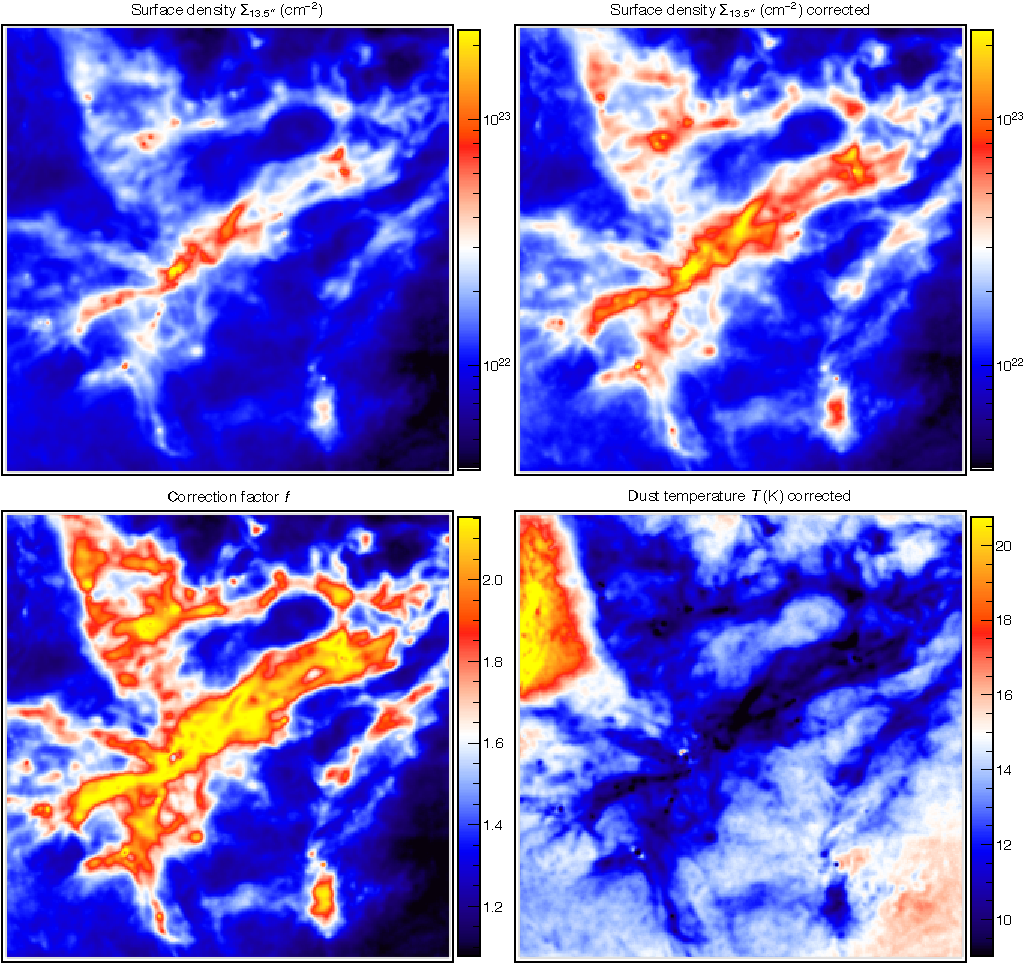
\includegraphics[width=\textwidth]{fig_aquila.pdf}
\caption{The Aquila field at $13.5{\arcsec}$ before and after the correction, on one common logarithmic scale, with the
correction factor and the dust temperature implied by the corrected surface density. The factor follows the structures: it is
least in the diffuse material between them and greatest along the ridges of the filaments and at the cores, which is where the
reconstruction is furthest from the truth and where masses are measured.}
\label{fig:aquila}
\end{figure*}

Figure~\ref{fig:aquila} shows the field before and after the correction, together with the factor and the dust temperature that
follows from the corrected surface density. The factor is not a uniform rescaling: it is smallest in the diffuse material between
the structures and largest along the ridges of the filaments and at the cores, so the contrast of the image rises as well as its
overall level. The dust of Aquila is heated by a field stronger than $G_0 = 10$ in places, most obviously in the warm corner at the upper
left of the temperature map, and the uncertainty this adds is discussed in Sect.~\ref{sec:field}.

% =====================================================================

\section{Uncertainties and limitations}
\label{sec:limits}

The first term below affects the measurement of a source rather than the correction itself, but it is the largest for the
masses of cores, which are what the correction is mostly used for. The others are uncertainties of the correction.

\subsection{The background and the footprint}
\label{sec:bgerr}

The mass of a core is the surface density within its footprint less the background beneath it, and neither the footprint nor the
background is known in a real image. Section~\ref{sec:valgrid} measured how much this matters on models whose backgrounds are as
simple as a background can be: a footprint misjudged by a quarter of its radius changes the median mass by $-15$ to $+9$ percent,
and by half its radius by $-47$ to $+18$ percent, with a spread over the models that widens sharply for footprints that are too
large. In a real cloud, a core lies on filaments and among other cores, the background beneath it is not the smooth continuation of
its surroundings \citep{Menshchikov2016}, and the errors are larger; they are discussed in Sect.~3.4.7 of
\citet{Menshchikov2021method} and Sect.~4.4 of \citet{Menshchikov2023}. None of this is changed by the correction, which acts on
the image and not on the source. It is the dominant uncertainty of a core mass, and it is the reason we preferred the simplest
correction to the more elaborate ones of Appendix~\ref{app:tcorr}: none of them changed the median mass of a core by more than a
few percent, which is well below this term.

\subsection{The radiation field}
\label{sec:field}

The relation of Eq.~(\ref{eq:law}) and therefore the factor were calibrated for an interstellar radiation field of $G_0 = 10$. To
measure how much a different field matters, we computed the models of the grid for nine fields from $G_0 = 0.98$ to 483, in steps
of a factor of 2.17 (Appendix~\ref{app:field}), and compared the factor that each set of models requires with the one the
correction applies, at surface densities of $10^{22}$ to $10^{23}$\,cm$^{-2}$. In fields of $G_0 \approx 1$ to 2 the applied
factor is too large, and the corrected surface density too high, by up to 33{\%}. For $G_0 = 5$ to 100 the error is at most
about 20{\%}, and it is below 6{\%} at $G_0 = 10$ itself; in fields of a few tens the correction falls short by up to
17{\%}, and above $G_0 \approx 200$ it is again too large at the highest surface densities. Most nearby star-forming clouds
are heated by fields within a factor of a few of $G_0 = 10$; for clouds in much weaker or much stronger fields, the correction
should be calibrated anew on models computed for the appropriate field. We examined whether the field could instead be read from the
observed dust temperature, pixel by pixel, and found that it cannot: a pixel may be warmer than the relation predicts because it
is heated by a stronger field, which requires more correction, or because it lies on the flank of a structure or behind a warm
cirrus, which requires less (Appendix~\ref{app:tcorr}).

\subsection{The arrangement along the line of sight}

An observed line of sight is not one structure but several, at depths that no observation reveals, and the method replaces them
by a single uniform body of the same total surface density. Equation~(\ref{eq:invariance}) shows that this substitution is exact
in the plane-parallel limit, so the error it commits is confined to the escape of radiation across the line of sight.
Appendix~\ref{app:arrange} measures it in the two forms it takes. Concentrating a bounded structure raises the required correction
by 3{\%} at a central-to-edge density ratio of 10 and by up to 15{\%} at a ratio of $10^3$. Embedding a structure in a
cirrus changes it by $-15$ to $+11$ percent according to the depth at which the structure sits, without a preferred sign, and the
value the method applies falls inside that range at every surface density we examined. We take 15{\%} as the uncertainty from
this source. Section~\ref{sec:fails} shows what it looks like in an image: not a uniform offset but a pattern that follows the
structures, small on their crests and largest on their flanks. Unlike the other terms, it cannot be reduced by a better
calculation, because the depth of a structure within a cloud is not an observable.

\subsection{The temperature relation and its floor}

The magnitude of the correction rests on Eq.~(\ref{eq:law}), and in particular on the temperature $T_{\rm f} = 6.6$\,K that dust
approaches when it is shielded from the radiation field completely. The factor is very sensitive to it: lowering the floor by
1\,K raises the factor by 27{\%} at $10^{22}$\,cm$^{-2}$ and by about 60{\%} at a few $10^{22}$\,cm$^{-2}$, and raising
it by 1\,K lowers the factor by 12 and 25{\%}. The floor is therefore the term that most needs to be right. Fitted to all 2086
models, the relation describes their median temperature to 3.5{\%} up to an attenuating column of $10^{23}$\,cm$^{-2}$, and
the temperatures of the densest models approach $T_{\rm f}$ smoothly (Fig.~\ref{fig:shielding}); fitted to only 15 models, as in an
earlier stage of this work, it gave $T_{\rm f} = 6.2$\,K and factors up to 13{\%} larger. Above $10^{23}$\,cm$^{-2}$ the models
hold too little mass to constrain the relation. Observations of prestellar cores usually place their centers at 7 to 9\,K, and an
analytic relation in common use places the floor at 10\,K; a floor that high would lower the factor substantially at the highest
surface densities.

\subsection{The geometry}

The calculation needs a shape, and an observed field does not supply one. Figure~\ref{fig:relation} shows that this scarcely
matters: a uniform sphere and a uniform layer of the same surface density give corrections within 8{\%} of each other
everywhere, and within 4{\%} outside a narrow band near $10^{22}$\,cm$^{-2}$. We average the two and take half their
difference as the uncertainty, which is 4{\%} at most.

\subsection{What the correction does not do}

It acts on an image, not on a source: the subtraction of the background of a core and the definition of its footprint are left to
the method that extracts the source. It also assumes that the dust is heated from outside, as in the models. A line of sight
through a protostar contains an internal source, its temperature gradient is reversed, and Eq.~(\ref{eq:correction}) does not
apply; such positions should be identified from their compact 70{\um} emission and left uncorrected.

% =====================================================================

\section{Conclusions}
\label{sec:conclusions}

The surface density images of molecular clouds derived by fitting one modified blackbody per pixel are systematically too low
wherever the dust temperature varies along the line of sight, and the deficit reaches a factor of three in the densest material.

The deficit cannot be measured from the observed colors. Its signature in the spectral energy distribution is 1 to 6{\%} of the
intensities where the deficit itself is 9 to 38{\%}, so any method that infers one from the other amplifies photometric errors
by a factor of 7 to 9, well beyond the accuracy of \emph{Herschel} photometry. The correction has to come from radiative transfer.

What radiative transfer supplies is a single relation between the dust temperature and the effective column of material that
shields the dust, which describes 102\,464 shells of 2086 models of embedded Bonnor--Ebert spheres with a mass-weighted scatter of
5.6{\%}. Size and concentration enter only through the shielding column, which is an average over the directions from which
the radiation arrives; a sphere, a cube and a plane-parallel layer of the same surface density then give correction factors within
10{\%} of one another. The relation gives the correction factor as an explicit function of the surface density that an image
holds, with no fitted parameters.

The correction is a correction of an image. It applies to a conventional surface density map at the resolution of the longest
waveband and to every image of a multi-resolution reconstruction, in which the deficit is the same fraction of the surface density
at every resolution. We evaluate it on the finest image of the reconstruction, which gives the sharpest corrected images and, on
radiative transfer models, the most accurate masses.

On 1815 radiative transfer models that were not used in the calibration, the correction raises the median mass of a core from 0.63
to 0.96 of the true value and the total surface density from 0.78 to 0.97, and it leaves the profile of a core within 2.5{\%}
of the truth beyond $20{\arcsec}$ from its center, with a deficit of 12{\%} remaining at the center. On a simulated sky of
cirrus, filaments and embedded cores, the masses of cores come out 9{\%} too high, because the diffuse background on which they
sit is over-corrected; the flanks of filaments are over-corrected by up to 30{\%}, so the slopes of filament profiles are
restored but not their widths or linear densities.

What the correction leaves in the mass of a core, a few percent in the median, is smaller than the error that a plausible
misjudgment of its footprint and background introduces, which is $-15$ to $+9$ percent for a footprint wrong by a quarter of its
radius even around the simplest models. This is why a correction that depends on the surface density alone is sufficient, and why
corrections that also read the fitted temperature, which cannot distinguish a stronger radiation field from the flank of a
structure, are not worth their complexity.

The correction is calibrated for $G_0 = 10$. Models computed for fields from $G_0 = 1$ to 500 show that it is accurate to about 20{\%}
 between $G_0 = 5$ and 100 and over-corrects by up to a third in the weakest fields. Its other uncertainties are the temperature
that fully shielded dust approaches, to which the factor is very sensitive above $10^{22}$\,cm$^{-2}$, and the arrangement of the
material along the line of sight, about 15{\%}, which is irreducible because the depth of a structure within a cloud is not an
observable. Applied to a field of the Aquila cloud, the correction raises the integrated surface density by a factor of 1.66 and
the number of pixels above $10^{23}$\,cm$^{-2}$ ninefold.

\begin{acknowledgements}
\draftnote{To be written.}
\end{acknowledgements}

\bibliographystyle{aa}
\bibliography{hires2_correction}

% =====================================================================

\appendix
\nolinenumbers 

\section{The grids of models}
\label{sec:grid}

All models are Bonnor--Ebert spheres embedded in a uniform spherical cloud and heated from outside by the interstellar radiation
field, computed with \emph{radmc-3d} for the dust of Sect.~\ref{sec:models}. Three grids were used, and Table~\ref{tab:grids}
summarizes them.

The main grid varies three parameters: the surface density of the embedding cloud $\Sig_{\rm emb}$, in steps of a factor of two
from $3.75\times10^{20}$ to $9.6\times10^{22}$\,cm$^{-2}$; the half-maximum size of the Bonnor--Ebert sphere, from 0.02 to
0.25\,pc; and its central-to-edge density ratio, from nearly uniform ($\rho_{\rm c}/\rho_{\rm e} \approx 1.2$) to strongly
concentrated ($\sim 10^3$). \draftnote{Please check these ranges and the numbers of steps along each axis.} Three further models,
built to extend the grid to $\Sig_{\rm emb}$ of $1.9$ to $7.9\times10^{23}$\,cm$^{-2}$, are optically thick in the far infrared
and are left out of the calibration (Sect.~\ref{sec:models}). The temperature structure of each model, tabulated shell by shell,
enters the relation of Eq.~(\ref{eq:law}).

The subdivision grid places its models between the nodes of the main grid, so that it tests the correction on models that did not
enter the relation. For each of its models, the intensities at 70 to 500{\um} were convolved to the beams of the wavebands,
reconstructed by \emph{hires} and corrected, and the true surface density was convolved to the same resolutions; the footprint of
the model is the area of the convolved true image that stands above the embedding cloud.

The grid of radiation fields repeats 305 models of the main grid, together with 34 models at a tenth embedding surface density of
$1.92\times10^{23}$\,cm$^{-2}$, for nine strengths of the interstellar radiation field from $G_0 = 0.98$ to 483, in steps of a
factor of 2.17. The lowest field is the weakest the implementation of the radiation field allows. About five models per field,
which required the largest images, were not computed; they do not affect the results of Appendix~\ref{app:field}.

\begin{table}
\caption{The grids of radiative transfer models.}
\label{tab:grids}
\centering
\begin{tabular}{lccl}
\hline\hline
\noalign{\smallskip}
Grid & $G_0$ & Models & Used for \\
\noalign{\smallskip}
\hline
\noalign{\smallskip}
Main          & 10           & 2089          & the relation of Eq.~(\ref{eq:law}) \\
Subdivision   & 10           & 1815          & validation, Sect.~\ref{sec:valgrid} \\
Radiation fields & 0.98--483 & $9\times339$ & Appendix~\ref{app:field} \\
\noalign{\smallskip}
\hline
\end{tabular}
\end{table}

\section{The arrangement of the material along the line of sight}
\label{app:arrange}

The correction is applied pixel by pixel, and a pixel receives the emission of everything along its line of sight. A single
modified blackbody is fitted to that sum, so what biases the fit is the whole distribution of dust temperatures along the line of
sight and not the temperature of any one structure within it. The method replaces that distribution by the one that a single
uniform body of the same total surface density would have. This appendix measures what the replacement costs.

\subsection{The invariance}
\label{app:invariance}

For a plane-parallel geometry the emergent emission depends on the total surface density alone. The attenuating column of a parcel is
determined by the column lying between it and each surface, which does not depend on how that column is distributed, and the mass
of a line of sight per unit column is constant for any density profile, which is Eq.~(\ref{eq:invariance}). As a check on the
algebra and on the integrations, we computed the four intensities of a line of sight of $2{\times}10^{22}$\,cm$^{-2}$ carrying a
clump thirty times the ambient density, placed at 15, 50 and 85{\%} of the depth. They differ from the smooth line of sight
of the same total surface density by at most $2.1{\times}10^{-4}$, $4.6{\times}10^{-5}$ and $1.2{\times}10^{-4}$, which is the accuracy of
the quadrature. Neither the concentration of the material nor the position of the clump has any effect at all.

\subsection{Concentration}
\label{app:concentr}

Since the density profile leaves the problem entirely in the plane-parallel limit, concentration can act only through the escape
of radiation across the line of sight, which a bounded structure permits and a layer does not. We measure it on a sphere of
density $\rho(r) \propto (1 + r^2/a^2)^{-1}$ out to its boundary, normalized so that the column through its center is the
observed one, with $a$ fixed by the central-to-edge density ratio. The parcels of the central line of sight are weighted by their
density, which is how the emission of that line of sight weights them, and the column that each of them must send its radiation
through is integrated along the ray to the boundary in every direction of the average.

\begin{table}
\caption{Correction factor required by the central line of sight of a sphere of the given central surface density, for four
central-to-edge density ratios. The first column is the uniform sphere that the method assumes.}
\label{tab:concentr}
\centering
\begin{tabular}{lcccc}
\hline\hline
\noalign{\smallskip}
$\Sig$ (cm$^{-2}$) & uniform & $10$ & $10^2$ & $10^3$ \\
\noalign{\smallskip}
\hline
\noalign{\smallskip}
$5{\times}10^{21}$ & 1.068 & 1.096 & 1.122 & 1.136 \\
$1{\times}10^{22}$ & 1.218 & 1.260 & 1.316 & 1.351 \\
$3{\times}10^{22}$ & 1.709 & 1.750 & 1.857 & 1.968 \\
$1{\times}10^{23}$ & 2.288 & 2.327 & 2.438 & 2.635 \\
\noalign{\smallskip}
\hline
\end{tabular}
\end{table}

Table~\ref{tab:concentr} gives the result. Concentration always raises the required correction, because the mass of a
concentrated structure sits where the shielding is deepest, and the effect grows with the surface density, from 3{\%} at a ratio of
10 to 15{\%} at a ratio of $10^3$. It is bounded and one-sided, so a correction built on uniform structures underestimates
the deficit of a concentrated one and never the reverse.

\subsection{Two superposed components}
\label{app:twocomp}

The second form of the question is a line of sight crossing a diffuse cirrus with a denser structure embedded in it at an unknown
depth. We take a plane-parallel cirrus of surface density $\Sig_{\rm c}$, in which the material at the column depth $x$ is shielded by the
angular average of $x/|\mu|$ toward the observer and $(\Sig_{\rm c} - x)/|\mu|$ away from it, and a uniform sphere whose surface density
through its center is $\Sig_{\rm s}$, embedded in that cirrus with the fraction $q$ of the surface density of the cirrus in front of it. A parcel
at the signed position $z$ along the diameter of the sphere, in units of its radius, is shielded by its own sphere over the path
\begin{equation}
   l(z,\psi) = -z\cos\psi + \sqrt{1 - z^2\sin^2\psi} ,
\label{eq:lsphere}
\end{equation}
in units of that radius, and by the cirrus over $q\,\Sig_{\rm c}/|\cos\psi|$ toward the observer and
$(1-q)\,\Sig_{\rm c}/|\cos\psi|$ away from it. The sign of $z$ has to be kept: with $|z|$ in its place the sphere would be
symmetric about its center whatever lay in front of it, and the answer would be wrong for every $q$ but one half. The angular
average of Eq.~(\ref{eq:seff}) is then taken over $\psi$ with the isotropic weight $\sin\psi$, the temperature of every parcel
follows from Eq.~(\ref{eq:law}), the emission of the cirrus and of the sphere are added with their masses, and one modified
blackbody is fitted to the sum exactly as the reconstruction fits it. The correction factor is the ratio of the true surface density to
the fitted one, as in Eq.~(\ref{eq:factor}). The construction is symmetric under $q \rightarrow 1-q$, as it must be, and the
computed factors are.

\begin{figure*}
\centering
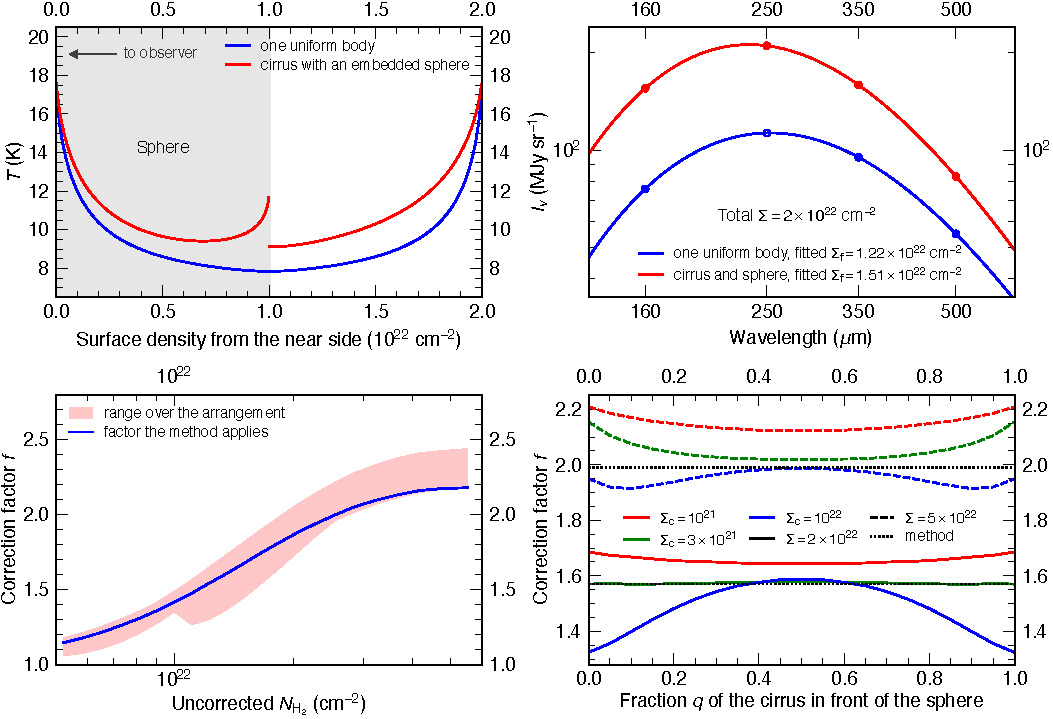
\includegraphics[width=0.9\textwidth]{fig_superposition.pdf}
\caption{\emph{Upper left}: the dust temperature along a line of sight of $2{\times}10^{22}$\,cm$^{-2}$, as the method assumes it
and as it would be if half of that surface density were a cirrus and half a uniform sphere pressed against its near face. The sphere is
warmer because it loses radiation across the line of sight and has nothing in front of it. \emph{Upper right}: the emission that
follows, with the single modified blackbody fitted to each, and the surface density that each fit returns. The two lines of sight
carry identical surface densities and nothing observable distinguishes them. \emph{Lower left}: the correction factor, the curve that the
method applies and the range spanned by embedding a sphere in a cirrus of $10^{21}$, $3{\times}10^{21}$ and
$10^{22}$\,cm$^{-2}$ at every position within it. \emph{Lower right}: the same factor against the fraction $q$ of the cirrus
lying in front of the structure, symmetric about $q = 0.5$ as it must be, with the value the method applies dotted.}
\label{fig:superposition}
\end{figure*}

Figure~\ref{fig:superposition} gives the result. The departure from the value that the method applies runs from $-15$ to
$+11${\%}, it has no preferred sign, and the value of the method lies inside the range spanned by the arrangement at every
surface density.
The spread is largest, 20{\%}, when the diffuse component carries half of the surface density, and it is below 10{\%} in most of
the configurations examined. The lower right panel shows the dependence on the depth at which the structure sits: it is symmetric
about the mid-plane, as it must be, and weakest when the diffuse component is a small part of the surface density.

The middle panel of Fig.~\ref{fig:superposition} shows why the effect exists at all, and that it is a property of the fit rather
than of the geometry. The two lines of sight drawn there carry exactly the same total surface density, but in one of them half of it is a
sphere at the near face of the cirrus, where it loses radiation sideways and has nothing in front of it to block the incoming
field. That arrangement is warmer, it is brighter in all four wavebands, and the single modified blackbody fitted to it returns
$1.54{\times}10^{22}$\,cm$^{-2}$ where the uniform body returns $1.30{\times}10^{22}$\,cm$^{-2}$. The same true surface density would
then need a correction of 1.30 rather than 1.54.

Nothing observable distinguishes the two. The depth of a structure within a cloud is not a measurable quantity and no improvement
of the calculation can recover it, so the 15{\%} of Sect.~\ref{sec:limits} is an irreducible uncertainty of any method of
this kind rather than a defect of this one.

\section{Why the observed colors cannot supply the correction}
\label{app:colors}
\label{sec:amplification}

It is natural to attempt to measure the temperature structure directly, by fitting more than one component to the observed
spectral energy distribution of each line of sight. Without noise this works: a free two-temperature fit over 160 to 500{\um}
recovers between 0.96 and 1.00 of the true surface density at the center of the four models, against 0.62 to 0.91 for the
single-temperature fit. With noise it does not. The reason is quantitative and is set out in Table~\ref{tab:signature}.

\begin{table}
\caption{Signature of the temperature mixing in the four-band spectral energy distribution at the center of each model, compared
with the deficit it produces. Columns two to five give the relative residuals, in percent, of the best single-component fit to the
noiseless intensities; column six their root-mean-square; column seven the fraction of the true surface density that the
single-component fit recovers.}
\label{tab:signature}
\centering
\begin{tabular}{lcccccc}
\hline\hline
\noalign{\smallskip}
$\rho_{\rm c}/\rho_{\rm e}$ & 160 & 250 & 350 & 500 & rms & recovered \\
\noalign{\smallskip}
\hline
\noalign{\smallskip}
1.18  & $+0.92$ & $-1.37$ & $-0.44$ & $+0.93$ & 0.97 & 0.914 \\
1.28  & $+0.88$ & $-2.16$ & $-0.46$ & $+1.82$ & 1.50 & 0.869 \\
4.47  & $+3.46$ & $-6.44$ & $-1.56$ & $+5.39$ & 4.61 & 0.680 \\
90.8  & $+3.76$ & $-8.04$ & $-1.64$ & $+7.27$ & 5.79 & 0.619 \\
\noalign{\smallskip}
\hline
\end{tabular}
\end{table}

The residual pattern is the same at every model, positive at 160 and 500{\um} and negative at 250 and 350{\um}, which is the
broadening of the spectral energy distribution by a distribution of temperatures. Dividing the deficit by the root-mean-square of
the residuals gives 8.9, 8.7, 6.9 and 6.6: any scheme that infers the deficit from the band-to-band photometry amplifies
relative photometric errors by a factor of 7 to 9. The calibration uncertainties adopted for \emph{Herschel} observations of
Aquila are 20\% at 70 to 160{\um} and 10\% at 250 to 500{\um} \citep{Konyves+2015}, so at the two weakly concentrated models the
entire signature lies below the photometric accuracy. A test that accepts a second component only where it improves the fit
significantly never fires, at any pixel of any model.

\begin{figure*}
\centering
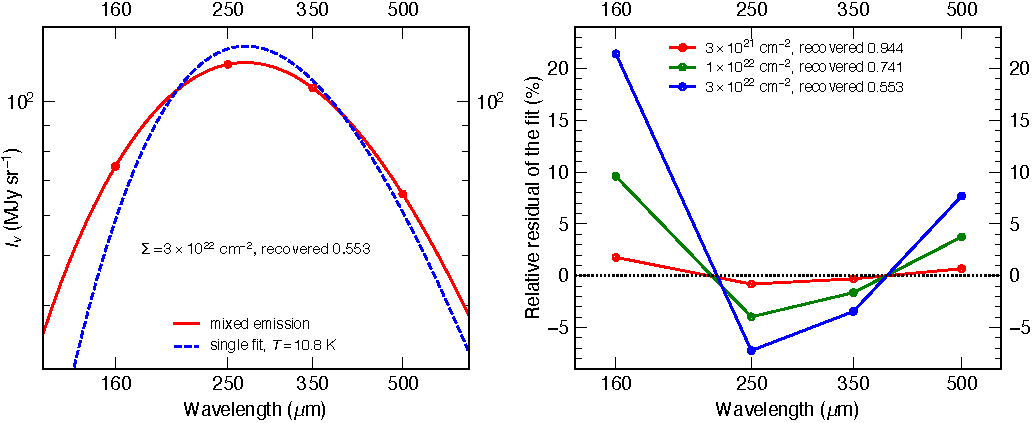
\includegraphics[width=0.9\textwidth]{fig_mixing.pdf}
\caption{\emph{Left}: the emission of a line of sight of $3{\times}10^{22}$\,cm$^{-2}$, the sum over depth of material at every
temperature, with the single modified blackbody fitted to it in the four wavebands and with the weights that the reconstruction
uses. The fit is drawn toward the warmer and brighter material, so the temperature it returns is too high and the surface density
that follows from it is too low. \emph{Right}: the relative residuals of that fit, waveband by waveband, for three total surface densities,
with the fraction of the true surface density recovered beside each. The pattern is always the same, positive at the ends and
negative in the middle, and it grows with the surface density, but it never rises above the calibration uncertainties of 20{\%} at
160{\um} and 10{\%} at the three longer wavebands.}
\label{fig:mixing}
\end{figure*}

Figure~\ref{fig:mixing} shows the whole of this in one place: the emission of a mixed line of sight, the single modified
blackbody that is fitted to it, and the residuals that remain. The correction must therefore be calibrated externally, on models
in which the answer is known.

\section{The radiation field}
\label{app:field}

The relation of Eq.~(\ref{eq:law}) was measured for a single field, $G_0 = 10$, and a stronger field heats the dust at every
attenuating column, which changes the deficit that the fit incurs. To measure how much, the correction was tested on the grid of
radiation fields of Appendix~\ref{sec:grid}. For each field, every pixel of every model was reconstructed and assigned to a cell of
fitted surface density, and in each cell we took the median, over the pixels, of the factor that restores the true surface density.
Table~\ref{tab:field} compares that factor with the one the correction applies, as the relative error of the corrected surface
density, the applied factor divided by the required one minus one.

\begin{table}
\caption{Relative error of the corrected surface density, in percent, for models computed in radiation fields of strength $G_0$,
in four ranges of the uncorrected surface density $\Sig$ (in cm$^{-2}$). Positive values mean that the correction is too large.
The values are medians over the pixels of all models of each field, weighted by the number of pixels.}
\label{tab:field}
\centering
\begin{tabular}{rcccc}
\hline\hline
\noalign{\smallskip}
$G_0$ & $\log\Sig$: 21.6--22.0 & 22.0--22.4 & 22.4--22.8 & 22.8--23.4 \\
\noalign{\smallskip}
\hline
\noalign{\smallskip}
0.98 & $+9$  & $+30$ & $+33$ & $+27$ \\
2.12 & $+9$  & $+24$ & $+28$ & $+22$ \\
4.61 & $+1$  & $+11$ & $+18$ & $+6$  \\
10   & $-4$  & $0$   & $+6$  & $-5$  \\
21.7 & $-10$ & $-12$ & $-2$  & $-8$  \\
47.1 & $-14$ & $-16$ & $-8$  & $-12$ \\
102  & $-17$ & $-10$ & $-2$  & $-3$  \\
222  & $-11$ & $-5$  & $+13$ & $+12$ \\
483  & $-6$  & $+4$  & $+28$ & $+30$ \\
\noalign{\smallskip}
\hline
\end{tabular}
\end{table}

The error changes sign twice: the correction is too large in the weakest fields, too small in fields of a few tens, and too large
again at the highest surface densities in the strongest fields. The deficit of a single-temperature fit depends on how the
temperature varies along the line of sight, not on the temperature itself, and a stronger field changes that variation
differently at different depths, so no simple rescaling of Eq.~(\ref{eq:law}) with the field reproduces the table. At $G_0 = 10$
the models of this grid reproduce the correction to 6{\%}, which confirms that the relation fitted to the main grid is not
specific to it.

A correction for a cloud in a field very different from $G_0 = 10$ therefore needs a relation measured in that field; the
procedure of Sect.~\ref{sec:law} applies unchanged. Estimating the field from the observed temperatures of the diffuse material
over scales of several arcminutes, where it varies, would be possible in a large map but not in a small one, in which most pixels
lie on structures (Appendix~\ref{app:tcorr}).

\section{Corrections that read the fitted temperature}
\label{app:tcorr}

The reconstruction writes a dust temperature beside every surface density, and a pixel whose temperature departs from what the
relation predicts at its surface density carries information that the surface density alone does not. We tested four ways of using
it, all calibrated on the radiative transfer models; none was adopted, and the reason is the same for all of them.

The first was a table of the required factor measured directly on the models, as a function of three observables: the surface
density, the fitted temperature and the contrast between the images at $13.5{\arcsec}$ and $36.3{\arcsec}$, which distinguishes the
crest of a structure from its flank. The second multiplied the factor of Eq.~(\ref{eq:factor}) by a smooth function of the surface
density and of the offset of the fitted temperature from the relation, fitted to the grid of radiation fields of
Appendix~\ref{app:field}; on the models it predicted the required factor to within 7{\%} in every field, and to within 6{\%}
 for a field left out of the fit. The third was a surface in surface density and temperature computed, like
Eq.~(\ref{eq:factor}), from analytic lines of sight through spheres, cylinders and layers embedded in a diffuse medium. The fourth
kept the factor of Eq.~(\ref{eq:factor}) but redistributed the correction within each beam of the coarsest image to follow the
shape of the finest one.

On the radiative transfer models of the subdivision grid, the first two raised the median mass of a core by 9 and 3{\%}
relative to the adopted correction, and the fourth changed it by 2{\%}; the third, tested on the grid of radiation fields,
under-corrected the dense material by a factor of 1.5 to 1.7 in fields of $G_0 = 20$ to 50. On the simulated sky, the first two
over-corrected the flanks of filaments more than the adopted correction does, by 39 to 43{\%} at $36{\arcsec}$ from the crest
against 28{\%}, and the first gave a correction factor visibly structured on the scale of its cells. The fourth narrowed the
filaments slightly and weakened the rings around extended cores, but not those around compact ones, and in the Aquila field it
imprinted the small-scale texture of the finest image, including its noise, onto the factor.

The reason is that a warm pixel is ambiguous. A pixel can be warmer than the relation predicts because a stronger radiation field
heats it, in which case the radiative transfer models say that it needs more correction; or because it lies on the flank of a
structure, close to its surface, or because its line of sight also crosses a warm cirrus, in which case it needs less. The models
used for the calibration contain only the first cause, and the simulated sky mostly the second, so a correction that reads the
temperature is right on one and wrong on the other. The fitted temperature of a single pixel cannot distinguish the two causes. A
field varies over parsecs and the warmth of a flank over the width of a filament, so the field could in principle be estimated from
the temperature of the diffuse material smoothed over several arcminutes; in the Aquila field, only 12{\%} of the pixels are
diffuse enough for that, and most of them lie in one corner, so the estimate would be an extrapolation over most of the field.
Given that none of these corrections changed the mass of a core by more than the error of the background (Sect.~\ref{sec:bgerr}),
we adopted the simplest.

\section{Filaments and cores on the simulated sky}
\label{app:filaments}

Table~\ref{tab:widths} gives the shape of the filaments of the simulated sky, measured on the median profile of each filament across
its length, and Fig.~\ref{fig:masses} the masses of cores and filaments. The level of the background beneath a filament is fitted
together with its profile, as the constant $B$ of $A\,r^{-\alpha} + B$ between $20{\arcsec}$ and $180{\arcsec}$ from the crest,
because the wings of these filaments fall so slowly that no radius within the spacing of the filaments reaches the background.

\begin{table}
\caption{Shape of the filaments of the simulated sky, as the median over the seven filaments: the half-maximum width $H$ above the
fitted background, the index $\alpha$ of the wings, the linear density $\Lambda$ within $\pm100{\arcsec}$ and the amplitude of the 
crest above the background, the last two as fractions of the true values. The filaments were built with a width of $40{\arcsec}$, 
which the beam of $13.5{\arcsec}$ broadens to about $42{\arcsec}$, and wings falling as $r^{-0.75}$.}
\label{tab:widths}
\centering
\begin{tabular}{lcccc}
\hline\hline
\noalign{\smallskip}
 &\!\!\!\! True &\!\!\!\! Uncorr. &\!\!\!\! Base $13.5{\arcsec}$ &\!\!\!\! Base $36.3{\arcsec}$\\
\noalign{\smallskip}
\hline
\noalign{\smallskip}
width $H$                  &\!\!\!\! $50.0{\arcsec}$ &\!\!\!\! $93.0{\arcsec}$ &\!\!\!\! $71.8{\arcsec}$ &\!\!\!\! $78.2{\arcsec}$\\
index $\alpha$             &\!\!\!\! 0.82            &\!\!\!\! 0.57            &\!\!\!\! 0.75            &\!\!\!\! 0.73\\
linear density $\Lambda$   &\!\!\!\! 1               &\!\!\!\! 0.87            &\!\!\!\! 1.47            &\!\!\!\! 1.44\\
crest amplitude            &\!\!\!\! 1               &\!\!\!\! 0.60            &\!\!\!\! 1.20            &\!\!\!\! 1.12\\
\noalign{\smallskip}
\hline
\end{tabular}
\end{table}

\begin{figure*}
\centering
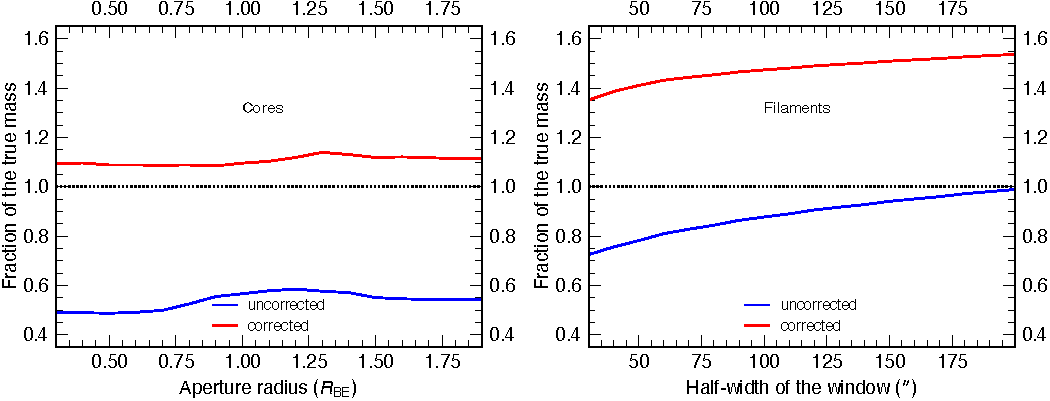
\includegraphics[width=0.9\textwidth]{fig_masses.pdf}
\caption{Masses recovered from the simulated sky, as fractions of the true values, before and after the correction with the base
at $13.5{\arcsec}$. \emph{Left}: the mass of a core, against the radius of the aperture in units of the Bonnor--Ebert radius, with
the background taken between 2 and 2.5 radii. \emph{Right}: the linear density $\Lambda$ of a filament, against the half-width of the
window over which the profile is integrated, above the fitted background. Both are medians, over the injected cores and over the
seven filaments.}
\label{fig:masses}
\end{figure*}

\begin{figure}
\centering
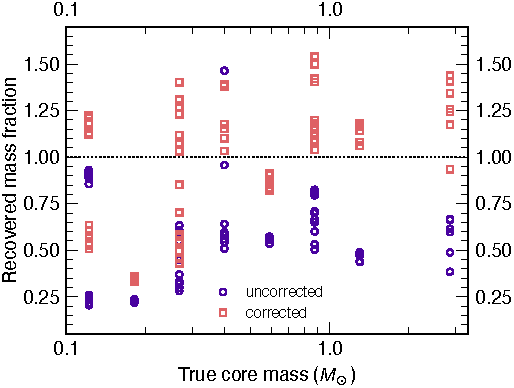
\includegraphics[width=0.9\columnwidth]{fig_core_recovery.pdf}
\caption{Integrated surface density of each injected core above its local background, as a fraction of the true value, before and
after the correction, against the true mass of the core. The dotted line marks a perfect recovery.}
\label{fig:cores}
\end{figure}

\begin{figure*}
\centering
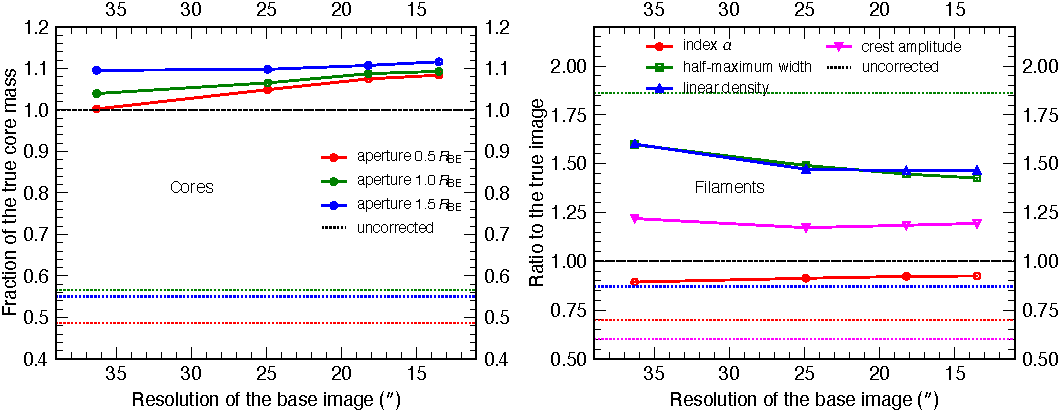
\includegraphics[width=\textwidth]{fig_base.pdf}
\caption{What the choice of the base image changes on the simulated sky. The factor is evaluated on the reconstruction at the
resolution on the abscissa and the correction is added to the image at $13.5{\arcsec}$, which is Eq.~(\ref{eq:correction}) with the
base taken in turn at each available resolution. \emph{Left}: the mass of a core recovered within three apertures, in units of the
Bonnor--Ebert radius. \emph{Right}: the shape of a filament, as ratios to the true image so that one axis serves for all four
quantities. Dotted lines mark the uncorrected reconstruction and the dashed line the true value.}
\label{fig:base}
\end{figure*}

The true image gives $\alpha = 0.82$ against the 0.75 with which the filaments were built, the excess coming from the beam and from
the flattening of the inner profile. The uncorrected reconstruction gives 0.57, far too shallow, because the crest is suppressed much
more than the wings, and the correction returns it to 0.75. The width is not restored: the uncorrected reconstruction makes the
filaments 86{\%} too wide, because the suppression of the crest flattens the profile, and after the correction they remain 44{\%} 
too wide, because the over-corrected flanks hold the profile open. For the same reason the linear density $\Lambda$ comes out
35 to 55{\%} too high, depending on the window (Fig.~\ref{fig:masses}, right). The cores are much less affected: their masses are
recovered with little dependence on the aperture out to one Bonnor--Ebert radius (Fig.~\ref{fig:masses}, left), and core by core
the recovered fraction of the mass above the background has a median of 1.12 after the correction, against 0.56 before it
(Fig.~\ref{fig:cores}).

Every curve of Fig.~\ref{fig:masses} is a ratio of the reconstruction to the truth measured by the identical procedure, so an
error of the background that affects the images alike cancels out of the ratio, and what the filament entries show is the
over-correction of the flanks and not the background. The absolute mass of a filament is another matter, and it is uncertain for 
reasons that have nothing
to do with the correction. Two of them act here. The first is a near-degeneracy: a constant and a tail falling as $r^{-0.75}$ are
almost the same function over any range that can be used, so the fitted level absorbs part of the filament. On these profiles the
fitted $B$ comes out at 0.65 to 0.80 of the true cirrus beneath the crest. The second is the curvature of the background itself.
A background that is convex over the extent of a filament lies above any chord drawn across it, so an interpolated level is too
low; and because that error is largest directly beneath the filament and vanishes at the interpolation points, it adds a centrally
peaked bump to the profile, which inflates the mass and steepens the measured index rather than merely shifting the zero point.
On the simulated cirrus a chord is accurate to better than 1{\%} over baselines up to $\pm600{\arcsec}$ and underestimates
the level by 13{\%} at $\pm900{\arcsec}$, so the effect is negligible for a core and grows with the extent of the structure.
A further difficulty, discussed by \citet{Menshchikov2016}, is that the background beneath a structure is not the smooth
continuation of its surroundings at all: removing the structure leaves an empty volume in its place, so the background that should
be subtracted has the shape of a crater. Detailed accounts of these problems are given in Sect.~3.4.7 of
\citet{Menshchikov2021method} and Sect.~4.4 of \citet{Menshchikov2023}. None of them is addressed by the correction, and none of
them is made worse by it.

A filament linear density $\Lambda$ obtained this way is uncertain at the level of tens of percent whether or not the correction is
applied, and improving it requires a better treatment of the background, not a better correction.

\section{Why the sphere and the layer are the limits}
\label{app:shape}

\begin{figure*}
\centering
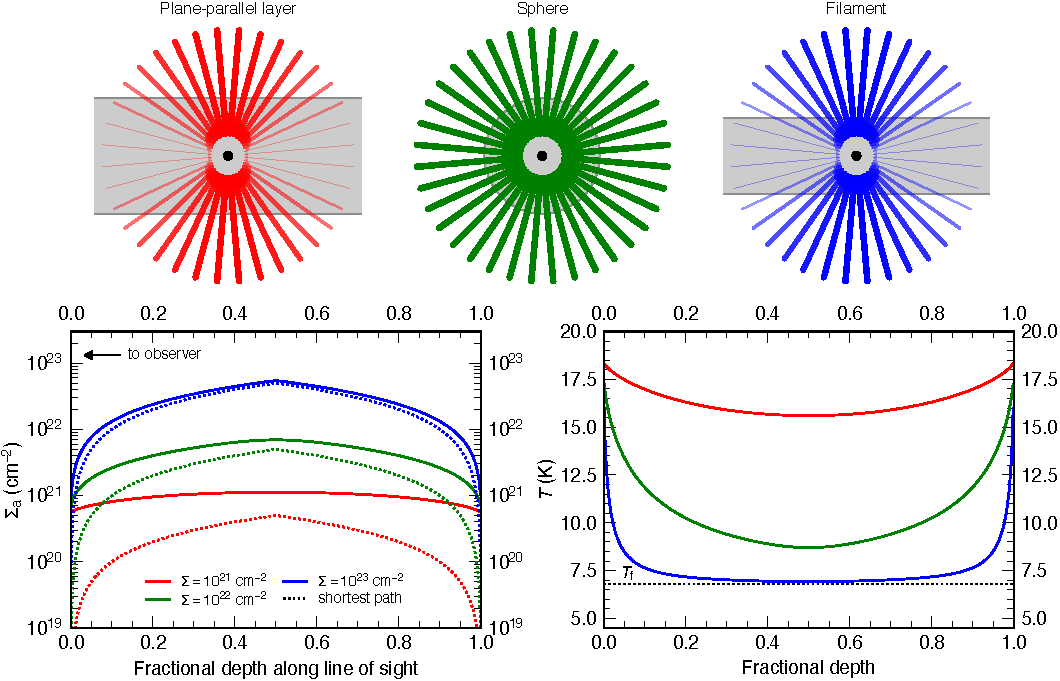
\includegraphics[width=0.8\linewidth]{fig_geometry.pdf}
\caption{\emph{Upper panels}: the radiation that heats a parcel of dust, marked by the black point, arrives from every direction
having crossed columns of very different length. The arrows are drawn thicker where less material has been crossed. In a layer
almost everything arrives along the normal; at the center of a sphere no direction is favored; a filament is intermediate, short
across and long along its axis. \emph{Lower panel}: the effective attenuating column of Eq.~(\ref{eq:seff}) along a line of sight
through a layer, as a fraction of the surface density the observer measures, for three total surface densities. The dotted line is 
what the shortest path alone would give.}
\label{fig:geometry}
\end{figure*}

The cube is in the figure to show that the two limits are limits. It is a body with none of the symmetry of either, and its
correction falls between them at every surface density, within 6{\%} of the sphere and 3{\%} of the layer at worst. A layer is
the extreme case and not one shape among several, and the reason is that it is unbounded across the line of sight. For a parcel at
its mid-plane the path to the boundary is the half-thickness divided by the cosine of the angle to the normal, so it diverges as
that angle approaches a right angle and a whole band of directions around the plane of the layer delivers nothing at all, however
thin the layer is made. At $10^{22}$\,cm$^{-2}$ the directions within $30\degr$ of the normal already carry 64{\%} of the
mean intensity and those within $45\degr$ carry 93{\%}. In a bounded body the path is finite in every direction, at most of
the order of the size of the body, and no direction is lost. A sphere is the opposite extreme, since a compact body of a given
central surface density blocks the least sky that any body of that surface density can. Every real cloud, of whatever outline, lies 
between the two, and the interval between them is the whole of what the shape can contribute. This is why the method needs no 
statement about the shape of the cloud it is applied to.

The dotted curve of Fig.~\ref{fig:relation} shows what is lost by ignoring the angular average altogether and using only the
column along the shortest path, with the geometric factor of one quarter that a sphere, a layer and a filament all share once
averaged over their bodies and over isotropic orientations. Below $3{\times}10^{21}$\,cm$^{-2}$ that cruder treatment agrees
with the full
calculation to 1{\%}, but it diverges above $10^{22}$\,cm$^{-2}$ and overestimates the correction by half at
$10^{23}$\,cm$^{-2}$. The shortest path assigns the deep material more shielding than it has, because the oblique directions
still deliver something, and the fit responds to the whole run of temperature and not to its extreme. The angular average is
therefore not a refinement of the shortest path but a different answer, and it is the one that the models support.

\end{document}
